% !TeX root = ../../Book3.tex
% 纲要标题：## 第6章　测地线变分、Jacobi 场与指标定理
% 纲要位置：几何学计划纲要.md，第 2324 行。
% 正文状态：初稿；尚未正式审核。

% 纲要内容开始
% 
% > 本章目标与证明范围：逐项导出端点项和指标形式，证明共轭点与二次变分的关系。路径空间语言只引入证明实际需要的部分，不以无限维直觉代替边值问题。
% 
% 纲要内容结束

\chapter{测地线变分、Jacobi 场与指标定理}
\label{g3:ch:06}
\BookChapterNumber{g3:ch:06}

\begin{chapterabstract}
	测地线是能量的驻定曲线，但走得足够远以后未必仍是最短曲线。本章从二参数变分逐项导出长度和能量的一、二次变分，保留固定端点与子流形端点各自的边界项。Jacobi 场描述邻近测地线的一阶变化，并把指数映射退化与共轭点联系起来。指标形式将这些微分方程与最短性连接；通过有限维分段测地线约化及共轭时刻的负定穿越，证明 Morse 指标等于开区间内共轭点重数之和。最后处理端点退化、焦点以及子流形起点的边界条件。
\end{chapterabstract}

\begin{learninggoals}
	\begin{itemize}
		\item 推导长度和能量的两次变分，说明端点项与曲率项的来源。
		\item 用 Jacobi 初值问题计算指数映射的微分、共轭点及其重数。
		\item 用指标形式检验局部极小性，区分割点与共轭点。
		\item 将分片光滑场约化到有限节点数据，计算指标跳跃与端点零空间。
		\item 从形算子导出子流形边界条件，并计算法向测地线的焦点。
	\end{itemize}
\end{learninggoals}

在圆球面上，从北极出发的不同经线最终会在南极相遇。在相遇以前，沿经线移动终点，邻近经线之间的横向间距先增大、后缩小，最后归零。这个横向间距的一阶变化由 Jacobi 场描述；归零说明指数映射失去一个可逆方向。若继续沿经线越过南极，则可以找到附近更短的连接曲线。要把这个现象变成定理，需要把测地线的微分方程与能量的二次变化放进同一个计算中。

\ProseParagraphBreak

整体最短性还有另一种失效方式。平坦圆柱上的两个点可能被绕圆柱两侧的同长测地线连接，虽然曲率为零、沿途也没有共轭点。二次变分检验的是给定曲线附近的变化，所有连接曲线的长度比较还会受到整体拓扑影响。本章先计算二次变化，再说明共轭点决定多少个下降方向，以及割点为何还可能来自另一条最短线。

\ProseParagraphBreak

直接所需基础是第一章的 Levi-Civita 联络、第二章的测地线初值问题、指数映射与完备性，以及第三章的曲率对称性；最后一小节另用第四章的第二基本形式和形算子。线性常微分方程的初值唯一性、对称矩阵的正负惯性及局部逆函数定理在使用处恢复所需内容。与本章对应的经典阅读材料是 Milnor 的第12--15节\cite[第12--15节，第70--87页]{Milnor1963Morse}；本章能量采用 \(\tfrac12\int|\dot\gamma|^2\)，其固定端点 Hessian 因而直接等于指标形式。证明只需要连续分片光滑变分及有限节点坐标，不预设路径空间上的无限维微分几何。

% !TeX root = ../../Book3.tex
% 纲要标题：### 6.1 长度与能量的变分
% 纲要位置：几何学计划纲要.md，第 2328 行。
% 正文状态：初稿；尚未正式审核。

% 纲要内容开始
% 
% * 变分场和协变导数交换
% * 第一变分及端点项
% * 第二变分和曲率项
% * 固定端点与自由端点的区别
% 
% 纲要内容结束

\section{长度与能量的变分}
\label{g3:sec:0601}

第二章用法邻域比较曲线长度，得到短测地线的极小性。现在固定一条曲线，把它向附近推开，考察长度先怎样变化、再怎样弯曲。一次变化检验曲线是否驻定，二次变化检验驻定曲线附近是否存在下降方向。端点是否允许移动会改变这两次计算的边界项，因而必须从一开始就说明允许哪些变分。

\subsection{变分场和协变导数交换}
\label{g3:subsec:0601:01}

设 \((M,g)\) 为光滑无边界黎曼流形，\(a<b\)。对光滑曲线 \(\gamma:[a,b]\to M\)，一个满足 \(F(0,t)=\gamma(t)\) 的光滑映射
\[
	F:(-\varepsilon,\varepsilon)\times[a,b]\longrightarrow M
\]
称为它的\term[quxian bianfen]{变分}[variation]。参数 \(s\) 选择附近的曲线，参数 \(t\) 沿每条曲线前进。记
\[
	T=\partial_tF,\qquad S=\partial_sF,\qquad V(t)=S(0,t).
\]
沿 \(\gamma\) 的向量场 \(V\) 称为\term[bianfen chang]{变分场}[variational vector field]。若 \(F(s,a),F(s,b)\) 分别恒等于 \(\gamma(a),\gamma(b)\)，就称变分固定端点。也允许 \(F\) 连续且在一个共同的有限 \(t\)-分割上分片光滑；每片均光滑到边界，各片的 \(s\)-导数在接缝处相同。这使变分场连续，而 \(D_tV\) 可以有跳跃。

\begin{figure}[htbp]
	\centering
	% !TeX root = ../Book3.tex
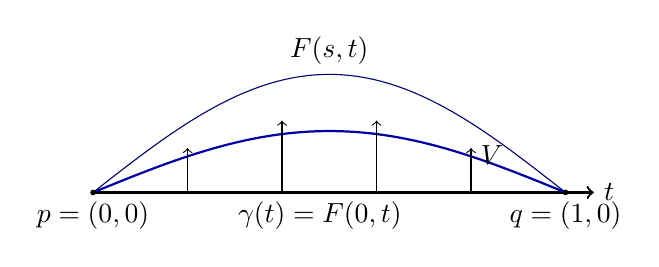
\begin{tikzpicture}[x=6cm,y=1.2cm]
	\draw[thick,->] (0,0)--(1.06,0) node[right] {\(t\)};
	\draw[blue!65!black,thick,domain=0:1,samples=60] plot (\x,{0.65*sin(180*\x)});
	\draw[blue!45!black,domain=0:1,samples=60] plot (\x,{1.25*sin(180*\x)});
	\foreach \x in {0.2,0.4,0.6,0.8}{
		\draw[->] (\x,0)--(\x,{0.8*sin(180*\x)});
	}
	\fill (0,0) circle[x radius=.006,y radius=.03];
	\fill (1,0) circle[x radius=.006,y radius=.03];
	\node[below] at (0,0) {\(p=(0,0)\)};
	\node[below] at (1,0) {\(q=(1,0)\)};
	\node[below] at (.48,0) {\(\gamma(t)=F(0,t)\)};
	\node[above] at (.5,1.25) {\(F(s,t)\)};
	\node[right] at (.8,.4) {\(V\)};
\end{tikzpicture}

	\caption{Euclid 平面上的固定端点变分 \(F(s,t)=(t,s\sin\pi t)\)。箭头表示沿水平基曲线的变分场 \(V=(0,\sin\pi t)\)，两端的场为零。}
	\label{g3:fig:fixed-endpoint-variation}
\end{figure}

沿 \(F\) 的协变导数使用拉回切丛。在任一坐标图中，若 \(Z=Z^k\partial_k|_F\)，则
\[
	(D_tZ)^k=\partial_tZ^k+\Gamma^k_{ij}(F)T^iZ^j,
	\qquad (D_sZ)^k=\partial_sZ^k+\Gamma^k_{ij}(F)S^iZ^j.
\]
因此这些运算不要求 \(F\) 是浸入，也不要求变分曲线互不相交。第二章证明 Gauss 引理时已经用过这种计算；现在还要交换两次协变导数。

\begin{proposition}\label{g3:prop:variation-commutation}
	设 \(F\) 是光滑无边界黎曼流形中的光滑二参数映射，\(T=\partial_tF\)、\(S=\partial_sF\)，\(Z\) 为沿 \(F\) 的光滑向量场。对 Levi-Civita 联络及本卷曲率约定，有
	\begin{equation}\label{g3:eq:variation-commutation}
		D_sT=D_tS,\qquad D_sD_tZ-D_tD_sZ=R(S,T)Z.
	\end{equation}
\end{proposition}
\begin{proof}
	第一式由 \(\partial_s\partial_tF^k=\partial_t\partial_sF^k\) 与 \(\Gamma^k_{ij}=\Gamma^k_{ji}\) 得到，即\eqref{g3:eq:mixed-variation-derivatives}。对第二式展开上面的两次导数，含 \(\partial_s\partial_tZ\)、一阶 \(Z\) 导数以及 \(\partial_sT^i-\partial_tS^i\) 的项相消。余项为
	\[
		\bigl(\partial_i\Gamma^k_{j\ell}-\partial_j\Gamma^k_{i\ell}
		+\Gamma^k_{ir}\Gamma^r_{j\ell}-\Gamma^k_{jr}\Gamma^r_{i\ell}\bigr)
		S^iT^jZ^\ell.
	\]
	由\eqref{g3:eq:curvature-coordinate-components}，这正是 \(R(S,T)Z\) 的第 \(k\) 个分量。
\end{proof}

任意沿 \(\gamma\) 的光滑场都能成为变分场。事实上，第二章的指数映射在零截面附近光滑；\([a,b]\) 紧，故对充分小的共同 \(s\)，可定义
\begin{equation}\label{g3:eq:exponential-field-variation}
	F(s,t)=\exp_{\gamma(t)}(sV(t)).
\end{equation}
由 \((\mathrm d\exp_x)_0=I\)，其变分场为 \(V\)。若 \(V(a)=V(b)=0\)，这个变分固定端点。连续分片光滑场也由同一公式实现为上述分片光滑变分。这里的紧性只涉及所给曲线的参数区间，无须假设整个 \(M\) 完备。

\subsection{第一变分及端点项}
\label{g3:subsec:0601:02}

对分片光滑曲线 \(c:[a,b]\to M\)，定义其\term[quxian nengliang]{能量}[energy]和长度
\begin{equation}\label{g3:eq:curve-energy-length}
	E(c)=\frac12\int_a^b|\dot c|^2\,\mathrm dt,
	\qquad L(c)=\int_a^b|\dot c|\,\mathrm dt.
\end{equation}
\symidx{\(E(c)\)：曲线能量}
长度在保向重参数化下不变，能量还记录行进速度。在固定区间上，Cauchy--Schwarz 不等式给出
\begin{equation}\label{g3:eq:energy-length-inequality}
	L(c)^2\le2(b-a)E(c),
\end{equation}
等号当且仅当速度长度几乎处处为同一个常数。特别地，若连接两端点的常速最短测地线 \(\gamma\) 存在，则
\[
	E(c)\ge \frac{L(c)^2}{2(b-a)}
	\ge\frac{d(\gamma(a),\gamma(b))^2}{2(b-a)}=E(\gamma).
\]
等号要求曲线同时最短且常速。使用能量可以保留测地线参数，又避开长度被积式在零速度处不可微的问题。

\begin{theorem}[第一变分]\label{g3:thm:curve-first-variation}
	设 \(F\) 是光滑无边界黎曼流形中光滑曲线 \(\gamma:[a,b]\to M\) 的光滑变分，\(V=\partial_sF|_{s=0}\)、\(T=\dot\gamma\)。则
	\begin{equation}\label{g3:eq:energy-first-variation}
		\left.\frac{\mathrm d}{\mathrm ds}E(F(s,\cdot))\right|_{s=0}
		=[\langle V,T\rangle]_a^b-\int_a^b\langle V,D_tT\rangle\,\mathrm dt.
	\end{equation}
	若 \(\gamma\) 正则，即 \(|T|>0\)，令 \(U=T/|T|\)，则
	\begin{equation}\label{g3:eq:length-first-variation}
		\left.\frac{\mathrm d}{\mathrm ds}L(F(s,\cdot))\right|_{s=0}
		=[\langle V,U\rangle]_a^b-\int_a^b\langle V,D_tU\rangle\,\mathrm dt.
	\end{equation}
\end{theorem}
\begin{proof}
	度量相容性和\cref{g3:prop:variation-commutation}给出
	\[
		\partial_s\tfrac12|\partial_tF|^2
		=\langle D_sT,T\rangle=\langle D_tS,T\rangle.
	\]
	对紧区间求导积分并分部积分，得到第一式。正则曲线的速度在紧区间上有正下界，所以充分小的变分也正则；此时
	\(\partial_s|T|=\langle D_tS,T/|T|\rangle\)。再次分部积分即得第二式。
\end{proof}

\begin{corollary}\label{g3:cor:energy-critical-geodesic}
	光滑无边界黎曼流形中的光滑曲线，在所有固定端点光滑变分下能量一阶导数为零，当且仅当它是仿射参数测地线。正则曲线在所有这样的变分下长度一阶导数为零，当且仅当它的弧长参数化是测地线。
\end{corollary}
\begin{proof}
	端点项为零。若第一式对所有端点为零的场 \(V\) 消失，取非负紧支函数 \(\chi\) 并用 \(V=\chi D_tT\)，得到 \(\int\chi|D_tT|^2=0\)，所以 \(D_tT=0\)。反向由公式直接成立。长度的情形以 \(D_tU\) 替代 \(D_tT\)，得到 \(D_tU=0\)。因为弧长 \(\ell\) 满足 \(\mathrm d\ell/\mathrm dt=|T|>0\)，这等价于 \(D_\ell U=0\)。
\end{proof}

对分片光滑的基曲线，逐片分部积分还会在每个内节点 \(t_i\) 出现项
\begin{equation}\label{g3:eq:energy-corner-terms}
	\langle V(t_i),T(t_i^-)-T(t_i^+)\rangle.
\end{equation}
允许独立移动节点后，能量驻定要求这些速度跳跃全部为零。长度公式则用单位切向量 \(U\) 的跳跃；它排除角点，但不要求两侧速度大小相等。这与第二章最短曲线可以按弧长参数化为光滑测地线的结论相符。

\subsection{第二变分和曲率项}
\label{g3:subsec:0601:03}

以下在仿射参数测地线处求二次变化。记 \(V'=D_tV\)，并令
\[
	A(t)=(D_sS)(0,t).
\]
\(A\) 是各条 \(s\)-曲线的协变加速度，通常并不为零。一次变分只看 \(V\)；若端点可动，二次变分还会看到端点轨迹的加速度。

\begin{theorem}[能量第二变分]\label{g3:thm:energy-second-variation}
	设 \(\gamma:[a,b]\to M\) 为光滑无边界黎曼流形中的仿射参数测地线，\(F\) 为它的光滑变分，\(V=\partial_sF|_0\)、\(A=D_s\partial_sF|_0\)、\(T=\dot\gamma\)。则
	\begin{equation}\label{g3:eq:energy-second-variation}
		E''(0)=\int_a^b\bigl(|V'|^2-\langle R(V,T)T,V\rangle\bigr)\,\mathrm dt
		+[\langle A,T\rangle]_a^b.
	\end{equation}
	若变分固定端点，最后一项为零。若变分仅沿一个共同有限分割分片光滑，且变分场连续，同式仍按各片积分成立。
\end{theorem}
\begin{proof}
	在变分上对 \(E'(s)=\int\langle D_tS,T\rangle\) 再求导，得
	\[
		E''(0)=\int_a^b\bigl(\langle D_sD_tS,T\rangle+|D_tS|^2\bigr)\big|_{s=0}\,\mathrm dt.
	\]
	交换公式将第一项写成 \(\langle D_tA+R(V,T)V,T\rangle\)。由于 \(D_tT=0\)，对 \(D_tA\) 分部积分只留下端点项。\cref{g3:prop:curvature-symmetries}的斜伴随性质给出
	\[
		\langle R(V,T)V,T\rangle=-\langle R(V,T)T,V\rangle,
	\]
	于是得到所述公式。固定端点时，端点的整条 \(s\)-曲线为常曲线，故 \(A(a)=A(b)=0\)。在分片情形，各接缝处的 \(A\) 连续，基曲线的 \(T\) 也连续，因此内节点的边界项相消。
\end{proof}

当 \(T\) 为单位向量且 \(V\perp T\) 时，曲率项为 \(K(V,T)|V|^2\)。正曲率减小二次变化，负曲率增大二次变化。这是随后共轭点与曲率比较出现相反效应的具体原因。

\ProseParagraphBreak

固定端点时，二次变化只取决于 \(V\)，与实现它的变分的二阶数据无关。极化得到对称双线性形式
\begin{equation}\label{g3:eq:index-form-introduction}
	I_\gamma(V,W)=\int_a^b\bigl(\langle V',W'\rangle
	-\langle R(V,T)T,W\rangle\bigr)\,\mathrm dt.
\end{equation}
曲率对称性保证 \(V\mapsto R(V,T)T\) 自伴，故这个形式确实对称。在固定端点的二参数变分中，混合二阶导数就是 \(I_\gamma(V,W)\)：可把前一公式用于参数平面中每条直线，再由极化恒等式恢复混合项。\secref{g3:sec:0603}将把它作为指标形式系统研究。

\begin{theorem}[长度第二变分]\label{g3:thm:length-second-variation}
	设 \(\gamma:[a,b]\to M\) 为光滑无边界黎曼流形中的单位速测地线，\(F\) 为光滑变分，\(V,A,T\) 如前一定理。令 \(V^\perp=V-\langle V,T\rangle T\)，则
	\begin{align}
		L''(0)&=\int_a^b\bigl(|V'|^2-\langle V',T\rangle^2
		-\langle R(V,T)T,V\rangle\bigr)\,\mathrm dt
		+[\langle A,T\rangle]_a^b\notag\\
		&=I_\gamma(V^\perp,V^\perp)+[\langle A,T\rangle]_a^b.
		\label{g3:eq:length-second-variation}
	\end{align}
\end{theorem}
\begin{proof}
	令 \(q(s,t)=|\partial_tF|^2\)。在 \(s=0\) 处 \(q=1\)，故
	\[
		\partial_s^2\sqrt q=\tfrac12\partial_s^2q-\tfrac14(\partial_sq)^2.
	\]
	第一项积分是能量第二变分，而 \(\partial_sq|_0=2\langle V',T\rangle\)，得到第一行。写 \(V=fT+V^\perp\)，利用 \(D_tT=0\) 可得 \(V'=f'T+(V^\perp)'\)，其中后项仍垂直于 \(T\)。又因 \(R(T,T)=0\) 及 \(R(V^\perp,T)T\perp T\)，曲率项也只看 \(V^\perp\)，于是得到第二行。
\end{proof}

例如在 Euclid 空间中取单位直线段 \(\gamma\)，令 \(f(a)=f(b)=0\)。变分 \(F(s,t)=\gamma(t+sf(t))\) 在小 \(s\) 时只是重参数化，故长度恒定；其变分场是 \(V=fT\)，能量二次变化却为 \(\int_a^b(f')^2\)。长度的切向零方向来自参数自由度，不能将这些方向误认为几何上的共轭方向。

\subsection{固定端点与自由端点的区别}
\label{g3:subsec:0601:04}

现在允许起点在光滑嵌入子流形 \(P\) 内移动、终点在光滑嵌入子流形 \(Q\) 内移动。允许的场满足
\[
	V(a)\in T_{\gamma(a)}P,\qquad V(b)\in T_{\gamma(b)}Q.
\]
这些条件也足以实现变分。为说明这一点，在 \(P,Q\) 内选端点曲线 \(p(s),q(s)\)，其初速度分别是 \(V(a),V(b)\)。先用\eqref{g3:eq:exponential-field-variation}，再在指数映射的输入中加入两端的修正：用沿 \(\gamma\) 的平行运输，把
\[
	\eta_a(s)=\exp_{\gamma(a)}^{-1}p(s)-sV(a),\qquad
	\eta_b(s)=\exp_{\gamma(b)}^{-1}q(s)-sV(b)
\]
分别延到两端的短邻域，并乘以在相应端点为1、另一端附近为0的光滑截断函数。因为 \(\eta_a,\eta_b=O(s^2)\)，修正不改变变分场，却使端点恰落在 \(P,Q\) 上。这个构造也适用于连续分片光滑场。

\begin{proposition}\label{g3:prop:submanifold-endpoint-variation}
	设 \(P,Q\) 为光滑无边界黎曼流形 \((M,g)\) 的光滑嵌入子流形。光滑曲线 \(\gamma:[a,b]\to M\) 的两端分别在 \(P,Q\) 上。它在所有端点留在 \(P,Q\) 的变分下能量驻定，当且仅当它是测地线，且
	\[
		\dot\gamma(a)\perp T_{\gamma(a)}P,\qquad
		\dot\gamma(b)\perp T_{\gamma(b)}Q.
	\]
	在这样的测地线处，第二变分为
	\begin{equation}\label{g3:eq:submanifold-endpoint-hessian}
		E''(0)=I_\gamma(V,V)
		+\langle B^Q(V(b),V(b)),T(b)\rangle
		-\langle B^P(V(a),V(a)),T(a)\rangle,
	\end{equation}
	其中 \(B^P,B^Q\) 为第四章约定的环境法丛值第二基本形式。
\end{proposition}
\begin{proof}
	先取端点为零的场，由\cref{g3:cor:energy-critical-geodesic}得到测地线方程。再独立取两个端点的任意切向量，第一变分的边界项对它们都为零恰好等价于两端的正交性。反向同样由第一变分成立。

	起点轨迹 \(p(s)\) 位于 \(P\)，由\cref{g3:prop:gauss-decomposition}，其环境加速度的法向部分为 \(B^P(V(a),V(a))\)。切向部分与 \(T(a)\) 正交，因此
	\(\langle A(a),T(a)\rangle=\langle B^P(V(a),V(a)),T(a)\rangle\)。终点同理，代入能量第二变分即得公式。
\end{proof}

若只允许起点在 \(P\) 上移动而终点固定，则边界项化为
\[
	-\langle A_{T(a)}^P V(a),V(a)\rangle.
\]
这里形算子的约定是 \(\langle A_\nu X,Y\rangle=\langle B(X,Y),\nu\rangle\)，所以负号来自下端点的减号。\secref{g3:sec:0604}的焦点边界条件将由这一项导出。若“自由端点”指端点可在整个 \(M\) 中任意移动，则能量驻定要求该端速度为零；测地线速度恒定，因而只剩常曲线。非平凡自由边界问题须指定端点所在子流形。

\begin{example}\label{g3:exm:concentric-circles-boundary-hessian}
	在 Euclid 平面中取两条同心圆，半径分别为 \(r\) 和 \(r+\ell\)，其中 \(r,\ell>0\)。径向线段 \(\gamma(t)=(r+t,0)\)、\(0\le t\le\ell\)，垂直连接两圆。旋转变分
	\[
		F(s,t)=(r+t)(\cos s,\sin s)
	\]
	保持每条曲线的长度和能量，因此二次变化为零。其场 \(V=(r+t)e_2\) 却满足 \(I_\gamma(V,V)=\ell\)。按外法向计算，两个形算子分别为 \(-I/r\)、\(-I/(r+\ell)\)，所以边界修正为 \(-(r+\ell)+r=-\ell\)，恰好抵消积分项。这一计算同时核验了两端边界项的次序及形算子的符号。
\end{example}

% !TeX root = ../../Book3.tex
% 纲要标题：### 6.2 Jacobi 场与指数映射
% 纲要位置：几何学计划纲要.md，第 2335 行。
% 正文状态：初稿；尚未正式审核。

% 纲要内容开始
% 
% * Jacobi 方程的推导
% * 初值、Wronskian 配对与解空间
% * 指数映射的微分
% * 共轭点及其重数
% 
% 纲要内容结束

\section{Jacobi 场与指数映射}
\label{g3:sec:0602}

从同一点发出的直线，初始方向稍有改变，分离量便随时间线性增长；球面上从北极发出的经线，却会在南极重新相遇。要描述这种差别，可以让测地线的初始点和初速度随一个参数变化，再对这个参数求导。得到的向量场满足一个由曲率控制的线性方程，这就是 Jacobi\footnote{Carl Gustav Jacob Jacobi（1804--1851），德国数学家，研究椭圆函数、偏微分方程和分析力学。} 方程。它既描述测地线族的一阶分离，也计算指数映射的微分。

\subsection{Jacobi 方程的推导}
\label{g3:subsec:0602:01}

本节设 \((M,g)\) 为 \(n\) 维光滑无边界黎曼流形，\(\gamma:I\to M\) 是仿射参数测地线，\(I\) 为开区间。记 \(T=\dot\gamma\)，对沿 \(\gamma\) 的场简写 \(J'=D_tJ\)、\(J''=D_t^2J\)。特别地，\(T'=0\)。先设 \(F(s,t)\) 是一个光滑测地线变分：\(F(0,t)=\gamma(t)\)，且对每个固定的 \(s\)，曲线 \(t\mapsto F(s,t)\) 都满足测地线方程。令 \(S=\partial_sF\)、\(T_s=\partial_tF\)。由\cref{g3:prop:variation-commutation}，
\[
	0=D_sD_tT_s
	=D_tD_sT_s+R(S,T_s)T_s
	=D_t^2S+R(S,T_s)T_s.
\]
在 \(s=0\) 处取值，变分场 \(J(t)=S(0,t)\) 因而满足
\begin{equation}\label{g3:eq:jacobi-equation}
	J''+R(J,T)T=0.
\end{equation}
正号由本卷 \(R(X,Y)=\nabla_X\nabla_Y-\nabla_Y\nabla_X-\nabla_{[X,Y]}\) 的约定决定。例如正曲率球面上的法向分离量将满足振子方程，而不是指数增长方程。

\begin{definition}[Jacobi 场]\label{g3:def:jacobi-field}
	设 \(\gamma:I\to M\) 是光滑黎曼流形 \((M,g)\) 中的仿射参数测地线，\(T=\dot\gamma\)，\(D_t\) 为沿线协变导数，\(R\) 为 Levi-Civita 曲率。满足 Jacobi 方程 \(D_t^2J+R(J,T)T=0\)（式\eqref{g3:eq:jacobi-equation}）的光滑沿曲线向量场 \(J\)，称为沿 \(\gamma\) 的\term[Jacobi chang]{Jacobi 场}[Jacobi field]。全体这样的场构成实向量空间，记为 \(\mathcal J(\gamma)\)。
\end{definition}
\symidx{\(\mathcal J(\gamma)\)：沿测地线的 Jacobi 场空间}

刚才已经证明，测地线变分的变分场必为 Jacobi 场。反向命题也成立：给定一个 Jacobi 场，可以改变测地线的初始数据，使它成为所得到测地线族的变分场。这个构造依赖线性方程初值的唯一性，将在下一小节完成。

\ProseParagraphBreak

方程中的线性算子 \(\mathcal R_t:V\mapsto R(V,T)T\) 有两个关键性质。由曲率反对称性，它消去 \(T\)；由\cref{g3:prop:curvature-symmetries}的两对交换对称性，
\begin{equation}\label{g3:eq:jacobi-curvature-self-adjoint}
	\langle\mathcal R_tU,V\rangle
	=\mathrm{Rm}(U,T,V,T)
	=\mathrm{Rm}(V,T,U,T)
	=\langle U,\mathcal R_tV\rangle.
\end{equation}
因此 \(\mathcal R_t\) 自伴，而且保持 \(T^\perp\)。这使切向变化与法向变化能够分开处理，也将给出两个解之间的一个守恒配对。

\subsection{初值、Wronskian 配对与解空间}
\label{g3:subsec:0602:02}

二阶方程需要同时指定位置与一阶导数。这里的“位置”是沿测地线的向量 \(J(t_0)\)，一阶导数则是 \(J'(t_0)\)，二者都属于同一个切空间。

\begin{theorem}\label{g3:thm:jacobi-initial-data}
	下文 \(\mathcal J(\gamma)\) 表示沿 \(\gamma\) 的 Jacobi 场空间，撇号表示沿线 Levi-Civita 协变导数。
	设 \(\gamma:I\to M\) 为 \(n\) 维光滑黎曼流形中的仿射参数测地线，\(t_0\in I\)。对任意 \(v,w\in T_{\gamma(t_0)}M\)，存在唯一 \(J\in\mathcal J(\gamma)\) 满足
	\[
		J(t_0)=v,\qquad J'(t_0)=w.
	\]
	该解存在于整个 \(I\)，并线性依赖 \((v,w)\)。特别地，初值映射
	\begin{equation}\label{g3:eq:jacobi-initial-isomorphism}
		\mathcal J(\gamma)\longrightarrow
		T_{\gamma(t_0)}M\oplus T_{\gamma(t_0)}M,
		\qquad J\longmapsto(J(t_0),J'(t_0))
	\end{equation}
	是线性同构，故 \(\dim\mathcal J(\gamma)=2n\)。在光滑参数族中，解在共同的紧时间区间上光滑依赖测地线及初始数据。
\end{theorem}
\begin{proof}
	把 \(T_{\gamma(t_0)}M\) 的一个正交单位基沿 \(\gamma\) 平行移动，得到平行正交标架 \(e_1(t),\ldots,e_n(t)\)。所用存在性和参数依赖是第一卷第15章第2节“沿路径的平行移动”中的平行移动定理；在开区间上，先在包含 \(t_0\) 的紧子区间上构造，再由唯一性粘合。度量相容性保证标架始终正交。若 \(J=\sum_i j^ie_i\)，则 \(J'=\sum_i(j^i)'e_i\)，方程化为
	\begin{equation}\label{g3:eq:jacobi-matrix-equation}
		j''+\mathcal R(t)j=0,
		\qquad \mathcal R_{ij}(t)=\langle R(e_j,T)T,e_i\rangle.
	\end{equation}
	矩阵 \(\mathcal R(t)\) 光滑且对称。令 \(z=(j,j')^{\mathsf T}\)，便得到一阶线性系统
	\[
		z'=\begin{pmatrix}0&I_n\\-\mathcal R(t)&0\end{pmatrix}z.
	\]
	第一卷同节的“线性方程的全区间解”引理适用于这个 \(2n\) 阶系统，给出每个紧子区间上的唯一解、线性初值依赖及光滑参数依赖。用包含 \(t_0\) 的紧子区间穷尽 \(I\)，相邻解由唯一性一致，遂得到整个 \(I\) 上的解。初值映射的双射性和维数结论随即成立。对于参数族，在参数点附近先平滑选择初始正交标架，再作平行移动；上述矩阵系统的系数便光滑依赖参数，同一引理给出最后的断言。
\end{proof}

\begin{proposition}\label{g3:prop:jacobi-geodesic-variation}
	设 \((M,g)\) 为光滑无边界黎曼流形，\(J\) 为沿仿射参数测地线 \(\gamma:I\to M\) 的 Jacobi 场，\([a,b]\subset I\) 为紧区间。则存在 \(\varepsilon>0\) 和光滑测地线变分 \(F:(-\varepsilon,\varepsilon)\times[a,b]\to M\)，其中心曲线为 \(\gamma\)，变分场为 \(J\)。
\end{proposition}
\begin{proof}
	选 \(t_0\in[a,b]\)，记 \(p=\gamma(t_0)\)、\(v=J(t_0)\)、\(w=J'(t_0)\)。取 \(p(s)=\exp_p(sv)\)，并令 \(P_s:T_pM\to T_{p(s)}M\) 为沿这条短曲线从 \(0\) 到 \(s\) 的平行移动。定义初速度
	\[
		u(s)=P_s\bigl(T(t_0)+sw\bigr).
	\]
	于是 \(p'(0)=v\)，且沿 \(p(s)\) 的协变导数满足 \(D_su(0)=w\)。由\cref{g3:thm:geodesic-ivp}，取初始点 \(p(s)\)、初速度 \(u(s)\)，在时刻 \(t_0\) 出发，得到测地线族 \(F(s,t)\)。测地线流的定义域开，中心解的参数区间 \([a,b]\) 紧，故缩小 \(\varepsilon\) 后，所有这些曲线都在整个 \([a,b]\) 上存在并联合光滑。

	变分场 \(\widetilde J\) 满足 Jacobi 方程，且 \(\widetilde J(t_0)=v\)。交换一次协变导数还给出
	\[
		\widetilde J'(t_0)
		=D_t\partial_sF(0,t_0)
		=D_s\partial_tF(0,t_0)=D_su(0)=w.
	\]
	由\cref{g3:thm:jacobi-initial-data}，\(\widetilde J=J\)。
\end{proof}

给定 Jacobi 场以后，这个实现只需改变初始点和初速度。若要求变分中的测地线全都具有单位速度，还要额外满足 \(\langle J',T\rangle=0\)；下文的切向分解会说明这个量为何恒定。

\begin{proposition}\label{g3:prop:jacobi-wronskian}
	下文 \(\mathcal J(\gamma)\) 表示沿 \(\gamma\) 的 Jacobi 场空间，撇号表示沿线 Levi-Civita 协变导数。
	设 \((M^n,g)\) 为光滑黎曼流形，\(\gamma:I\to M\) 为仿射参数测地线，\(t_0\in I\)，\(J,K\) 是沿 \(\gamma\) 的 Jacobi 场。它们的\term[Wronskian peidui]{Wronskian 配对}[Wronskian pairing]\footnote{Józef Maria Hoëné-Wroński（1776--1853），波兰裔法国数学家、哲学家，其函数展开研究涉及后来称为 Wronskian 的行列式。}定义为
	\begin{equation}\label{g3:eq:jacobi-wronskian}
		W(J,K)=\langle J',K\rangle-\langle J,K'\rangle.
	\end{equation}
	右端与参数 \(t\) 无关，并在 \(\mathcal J(\gamma)\) 上给出非退化的交替双线性配对。对任一 \(t_0\)，子空间
	\[
		\mathcal J_{t_0}(\gamma)=\{J\in\mathcal J(\gamma):J(t_0)=0\}
	\]
	维数为 \(n\)，且其中任意两个场的 \(W\) 配对均为零。
\end{proposition}
\symidx{\(W(J,K)\)：Jacobi 场的 Wronskian 配对}
\begin{proof}
	由 Jacobi 方程及式\eqref{g3:eq:jacobi-curvature-self-adjoint}，
	\[
		\frac{\mathrm d}{\mathrm dt}
		\bigl(\langle J',K\rangle-\langle J,K'\rangle\bigr)
		=\langle-\mathcal R_tJ,K\rangle+\langle J,\mathcal R_tK\rangle=0.
	\]
	交替性和双线性由定义直接得到。在初值同构\eqref{g3:eq:jacobi-initial-isomorphism}下，若 \(J\) 对应 \((v,w)\)、\(K\) 对应 \((u,z)\)，则
	\[
		W(J,K)=\langle w,u\rangle-\langle v,z\rangle.
	\]
	如果此值对所有 \(K\) 都为零，取 \((u,z)=(w,-v)\)，可得 \(|w|^2+|v|^2=0\)，故 \(J=0\)。最后，\(J(t_0)=0\) 的场由任意 \(J'(t_0)\) 唯一决定，维数为 \(n\)；当 \(J,K\) 都在 \(t_0\) 消失时，在该时刻计算 \(W\) 即得零。
\end{proof}

\begin{proposition}\label{g3:prop:jacobi-tangential-normal}
	设 \((M,g)\) 为光滑黎曼流形，\(\gamma:I\to M\) 为单位速测地线，\(T=\dot\gamma\)，\(t_0\in I\)，撇号表示沿线协变导数。每个 Jacobi 场唯一分解为
	\begin{equation}\label{g3:eq:jacobi-tangential-normal}
		J(t)=\bigl(a+b(t-t_0)\bigr)T(t)+J^\perp(t),
		\qquad J^\perp(t)\perp T(t),
	\end{equation}
	其中 \(J^\perp\) 仍为 Jacobi 场，\(a=\langle J(t_0),T(t_0)\rangle\)、\(b=\langle J'(t_0),T(t_0)\rangle\)。特别地，\(J\) 处处垂直于 \(T\)，当且仅当这两个初始内积均为零；若 \(J\) 在两个不同时刻消失，则它处处垂直于 \(T\)。
\end{proposition}
\begin{proof}
	令 \(f=\langle J,T\rangle\)。因为 \(T'=0\)、\(\mathcal R_tT=0\) 且 \(\mathcal R_t\) 自伴，
	\[
		f''=\langle J'',T\rangle=-\langle\mathcal R_tJ,T\rangle=0.
	\]
	故 \(f(t)=a+b(t-t_0)\)。场 \(fT\) 满足 Jacobi 方程，因而 \(J-fT\) 也满足，并与 \(T\) 正交。其余结论来自一次函数的初值和零点性质。
\end{proof}

\begin{example}\label{g3:exm:constant-curvature-jacobi}
	设光滑黎曼流形 \((M,g)\) 具有常截面曲率 \(k\in\mathbb R\)，\(\gamma:I\to M\) 为单位速测地线，\(0\in I\)，\(T=\dot\gamma\)，撇号表示沿线协变导数。记从 \(0\) 到 \(t\) 的平行移动为 \(P_t\)，定义
	\begin{equation}\label{g3:eq:model-jacobi-functions}
		s_k(t)=
		\begin{cases}
			\sin(\sqrt{k}\,t)/\sqrt{k},&k>0,\\
			t,&k=0,\\
			\sinh(\sqrt{-k}\,t)/\sqrt{-k},&k<0,
		\end{cases}
		\qquad c_k(t)=s_k'(t).
	\end{equation}
	若 \(J(0)=aT(0)+u\)、\(J'(0)=bT(0)+v\)，其中 \(u,v\perp T(0)\)，则
	\begin{equation}\label{g3:eq:constant-curvature-jacobi-solution}
		J(t)=(a+bt)T(t)+P_t\bigl(c_k(t)u+s_k(t)v\bigr).
	\end{equation}
	事实上，常曲率公式\eqref{g3:eq:constant-sectional-algebraic}给出
	\[
		R(V,T)T=k\bigl(V-\langle V,T\rangle T\bigr).
	\]
	法向部分在平行标架中满足 \(j''+kj=0\)，而 \(c_k,s_k\) 的初值分别为 \((1,0)\)、\((0,1)\)。验证方程与初值后，\cref{g3:thm:jacobi-initial-data}即证明所列公式。由同一起点出发时 \(u=a=0\)，法向分离量由 \(s_k(t)\) 控制：正曲率下可以再次消失，零曲率下线性增长，负曲率下则含双曲正弦因子。
\end{example}
\symidx{\(s_k,c_k\)：常曲率 Jacobi 方程的标准解}

\subsection{指数映射的微分}
\label{g3:subsec:0602:03}

固定 \(p\in M\)。第二章已经定义指数映射 \(\exp_p:\mathcal E_p\to M\)，其中 \(\mathcal E_p\subset T_pM\) 为包含零的开星形集。要对 \(\exp_p\) 在向量 \(v\) 处沿 \(w\) 求导，只须改变初速度为 \(v+sw\)。这一变化恰好属于刚才研究的测地线变分。

\begin{proposition}\label{g3:prop:exponential-differential-jacobi}
	设 \((M,g)\) 为光滑无边界黎曼流形，\(\mathcal E_p\) 为指数映射 \(\exp_p\) 的定义域，撇号表示沿线协变导数。
	设 \(p\in M\)、\(v\in\mathcal E_p\)、\(w\in T_pM\)，令 \(\gamma_v(t)=\exp_p(tv)\)，\(0\le t\le1\)。沿此测地线取初值为
	\[
		J_w(0)=0,\qquad J_w'(0)=w
	\]
	的 Jacobi 场，则
	\begin{equation}\label{g3:eq:exponential-differential-jacobi}
		J_w(t)=(\mathrm d\exp_p)_{tv}(tw),
		\qquad (\mathrm d\exp_p)_v(w)=J_w(1).
	\end{equation}
	这里通过向量空间的自然平移，把 \(T_{tv}(T_pM)\) 识别为 \(T_pM\)。更一般地，若 \(\gamma(t)=\exp_p(tu)\) 定义在含 \(0\) 的区间上，\(J_w(0)=0\)、\(J_w'(0)=w\)，则对 \(t\ne0\) 有
	\begin{equation}\label{g3:eq:exponential-differential-time-scaling}
		(\mathrm d\exp_p)_{tu}(w)=\frac1tJ_w(t).
	\end{equation}
\end{proposition}
\begin{proof}
	由 \(\mathcal E_p\) 的开性，充分小的 \(s\) 满足 \(v+sw\in\mathcal E_p\)，星形性又保证
	\[
		F(s,t)=\exp_p\bigl(t(v+sw)\bigr),\qquad 0\le t\le1,
	\]
	有定义。对固定 \(s\)，这是初始速度为 \(v+sw\) 的测地线。其变分场 \(J\) 为 Jacobi 场，且因为 \(F(s,0)=p\)，有 \(J(0)=0\)。在起点交换导数，得到
	\[
		J'(0)=D_s\partial_tF(s,0)\big|_{s=0}
		=\left.\frac{\mathrm d}{\mathrm ds}(v+sw)\right|_{s=0}=w.
	\]
	唯一性说明 \(J=J_w\)，而链式法则给出 \(J(t)=(\mathrm d\exp_p)_{tv}(tw)\)。在 \(t=1\) 处即得第二式。对一般固定的 \(t\)，在包含 \(0,t\) 的紧区间上作同样的变分，或用测地线的仿射重参数化，得到 \(J_w(t)=(\mathrm d\exp_p)_{tu}(tw)\)；再用微分的线性性即得式\eqref{g3:eq:exponential-differential-time-scaling}。
\end{proof}

因子 \(1/t\) 记录了两种参数的区别：\(J_w'(0)=w\) 改变的是初速度，而在 \(tu\) 处取微分改变的是时间 \(t\) 后的指数映射自变量。沿径向取 \(w=u\) 时，唯一的初值解是 \(J_u(t)=t\dot\gamma(t)\)，因而
\[
	(\mathrm d\exp_p)_{tu}(u)=\dot\gamma(t).
\]
所以非零径向方向始终被映为非零向量。指数映射若发生奇异，原因必来自与径向正交的方向。

\begin{example}\label{g3:exm:model-exponential-differential}
	取 \(k\in\mathbb R\)。记 \(s_k\) 为 \(s_k''+ks_k=0\)、\(s_k(0)=0\)、\(s_k'(0)=1\) 的解，\(c_k=s_k'\)、\(\operatorname{ct}_k=c_k/s_k\)，\(b_k=\pi/\sqrt k\) 当 \(k>0\)，否则 \(b_k=\infty\)。
	在常曲率 \(k\) 的流形中，令 \(u\in T_pM\) 为单位向量，\(r>0\)，且测地线 \(\gamma(t)=\exp_p(tu)\) 定义到 \(r\)。对 \(w\perp u\)、\(a\in\mathbb R\)，\cref{g3:exm:constant-curvature-jacobi}及式\eqref{g3:eq:exponential-differential-time-scaling}给出
	\begin{equation}\label{g3:eq:model-exponential-differential}
		(\mathrm d\exp_p)_{ru}(au+w)
		=P_r\left(au+\frac{s_k(r)}r w\right).
	\end{equation}
	径向伸缩率为 \(1\)，横向伸缩率为 \(s_k(r)/r\)。当 \(r\to0\) 时，这个比值趋于 \(1\)，与 \((\mathrm d\exp_p)_0=I\) 相符。半径为 \(a_0\) 的圆球面上，它等于 \(a_0\sin(r/a_0)/r\)，在首次到达对径点时为零；平坦情形恒为 \(1\)。
\end{example}

\subsection{共轭点及其重数}
\label{g3:subsec:0602:04}

若一个非零 Jacobi 场在测地线段的两端都消失，它描述了端点在一阶上保持不动的测地线变化。这是后面指标型出现零方向的来源。定义必须保留所选的测地线段：同一对点可以由不同测地线连接，它们的线性化行为未必相同。

\begin{definition}[共轭点与重数]\label{g3:def:conjugate-point}
	设 \((M,g)\) 为光滑黎曼流形，\(\gamma:I\to M\) 是仿射参数测地线，\(\mathcal J(\gamma)\) 表示沿线 Jacobi 场空间，\(a,b\in I\)、\(a\ne b\)。若存在非零 Jacobi 场 \(J\) 满足 \(J(a)=J(b)=0\)，就称 \(\gamma(a)\) 与 \(\gamma(b)\) 沿该测地线段\term[gonge dian]{共轭}[conjugate]，并把
	\begin{equation}\label{g3:eq:conjugate-multiplicity}
		m_\gamma(a,b)
		=\dim\{J\in\mathcal J(\gamma):J(a)=J(b)=0\}
	\end{equation}
	称为该\term[gonge dian chongshu]{共轭点的重数}[multiplicity of a conjugate point]。固定 \(a\) 后，满足此条件的 \(b\) 称为相对 \(a\) 的共轭时刻。
\end{definition}
\symidx{\(m_\gamma(a,b)\)：沿指定测地线段的共轭重数}

非恒定测地线可以作常数倍重参数化成为单位速度曲线，而 Jacobi 方程在这种变换下保持形式。由\cref{g3:prop:jacobi-tangential-normal}，两端消失的 Jacobi 场必为法向场；它由起点的法向导数决定，故
\[
	0\le m_\gamma(a,b)\le n-1.
\]
恒定测地线上曲率项为零，平行标架中的解是一次函数，在两个不同时刻消失就只能为零。因此恒定测地线没有共轭时刻，一维黎曼流形中也没有共轭时刻。

\begin{proposition}\label{g3:prop:conjugate-exp-singularity}
	设 \((M,g)\) 为光滑无边界黎曼流形，\(\gamma:I\to M\) 为仿射参数测地线，\(m_\gamma\) 表示式\eqref{g3:eq:conjugate-multiplicity}的共轭重数，\(0\in I\)，\(p=\gamma(0)\)、\(u=\dot\gamma(0)\)。对 \(t_0\in I\setminus\{0\}\)，点 \(\gamma(t_0)\) 与 \(p\) 沿此段共轭，当且仅当 \((\mathrm d\exp_p)_{t_0u}\) 奇异，而且
	\begin{equation}\label{g3:eq:conjugate-exp-nullity}
		m_\gamma(0,t_0)=\dim\ker(\mathrm d\exp_p)_{t_0u}.
	\end{equation}
\end{proposition}
\begin{proof}
	满足 \(J(0)=0\) 的 Jacobi 场与初始导数 \(w=J'(0)\) 一一对应。由\cref{g3:prop:exponential-differential-jacobi}，
	\[
		J_w(t_0)=(\mathrm d\exp_p)_{t_0u}(t_0w).
	\]
	乘以非零数 \(t_0\) 是 \(T_pM\) 的同构，所以两边的核同维。定义立即给出结论。
\end{proof}

在非共轭时刻，逆函数定理保证所选初速度附近的测地线可以由终点光滑参数化。共轭时刻则存在非零的初速度变化，使终点的一阶变化为零。这一结论是线性化的陈述；它本身没有断言存在一族端点严格固定的不同测地线。

\begin{corollary}\label{g3:cor:jacobi-boundary-value}
	设 \((M,g)\) 为光滑无边界黎曼流形，\(a<b\)，\(\gamma:[a,b]\to M\) 为延拓到端点邻域的测地线，且两端沿此段不共轭。对任意 \(v\in T_{\gamma(a)}M\)、\(w\in T_{\gamma(b)}M\)，存在唯一 Jacobi 场满足 \(J(a)=v\)、\(J(b)=w\)。
\end{corollary}
\begin{proof}
	先取初值为 \((v,0)\) 的 Jacobi 场 \(J_0\)。映射
	\[
		T_{\gamma(a)}M\longrightarrow T_{\gamma(b)}M,
		\qquad z\longmapsto J_z(b),\quad
		J_z(a)=0,\quad J_z'(a)=z,
	\]
	的核由共轭定义为零；源和靶都是 \(n\) 维，所以它是同构。唯一选择 \(z\) 使 \(J_z(b)=w-J_0(b)\)，即可取 \(J=J_0+J_z\)。
\end{proof}

下一结论保证，在一个有限测地线段上，按重数逐个计数共轭时刻是有限过程。证明只使用光滑系数和初值唯一性，并不要求度量解析。

\begin{proposition}\label{g3:prop:conjugate-times-isolated}
	设 \(\gamma:I\to M\) 是光滑黎曼流形中的测地线，\(0\in I\)。相对 \(0\) 的每个共轭时刻在 \(I\) 中孤立；\(0\) 的某个穿孔邻域没有共轭时刻。因此每个紧子区间 \([a,b]\subset I\) 只含有限个相对 \(0\) 的共轭时刻，各自的重数有限。
\end{proposition}
\begin{proof}
	在沿 \(\gamma\) 的平行正交标架中，取矩阵方程
	\[
		Y''+\mathcal R(t)Y=0,\qquad Y(0)=0,\qquad Y'(0)=I_n.
	\]
	其第 \(i\) 列是初始导数为第 \(i\) 个基向量、初始值为零的 Jacobi 场。于是 \(t\ne0\) 为共轭时刻当且仅当 \(Y(t)\) 奇异，重数为 \(\dim\ker Y(t)\)。由 \(Y(t)=tI_n+O(t^2)\)，矩阵 \(Y(t)/t\) 趋于 \(I_n\)，所以 \(0\) 附近没有非零的共轭时刻。

	固定一个共轭时刻 \(t_0\ne0\)，写
	\[
		K=\ker Y(t_0),\qquad L=\operatorname{im}Y(t_0),
		\qquad C=L^\perp,\qquad m=\dim K=\dim C.
	\]
	Wronskian 配对在初始时刻为零，因而对所有 \(t\) 有
	\begin{equation}\label{g3:eq:jacobi-matrix-wronskian}
		Y(t)^{\mathsf T}Y'(t)=Y'(t)^{\mathsf T}Y(t).
	\end{equation}
	若 \(u\in K\)，则对任意 \(v\in\mathbb R^n\)，此式给出
	\[
		\langle Y'(t_0)u,Y(t_0)v\rangle
		=\langle Y(t_0)u,Y'(t_0)v\rangle=0.
	\]
	故 \(Y'(t_0)K\subset C\)。若还满足 \(Y'(t_0)u=0\)，则 Jacobi 场 \(Y(t)u\) 在 \(t_0\) 的值和导数都为零，由初值唯一性它恒为零，再在 \(0\) 处求导便得 \(u=0\)。维数相同于是说明
	\begin{equation}\label{g3:eq:jacobi-kernel-cokernel-isomorphism}
		B=Y'(t_0)|_K:K\longrightarrow C
	\end{equation}
	是同构。这是控制奇异时刻的关键：在消失的方向上，一阶导数恰好补满值域缺少的方向。

	现在按定义域 \(K^\perp\oplus K\) 和值域 \(L\oplus C\) 分块，令 \(\tau=t-t_0\)，写成
	\[
		Y(t)=\begin{pmatrix}A(t)&E(t)\\ F(t)&G(t)\end{pmatrix}.
	\]
	在 \(t_0\) 处，\(A(t_0):K^\perp\to L\) 可逆，其他三块均为零。Taylor 展开及式\eqref{g3:eq:jacobi-kernel-cokernel-isomorphism}给出
	\[
		E(t)=O(\tau),\qquad F(t)=O(\tau),\qquad
		G(t)=\tau B+O(\tau^2).
	\]
	当 \(t\) 接近 \(t_0\) 时，\(A(t)\) 仍可逆。以可逆块矩阵作消元，\(Y(t)\) 可逆等价于下面的补块可逆：
	\begin{equation}\label{g3:eq:jacobi-singular-block}
		G(t)-F(t)A(t)^{-1}E(t)
		=\tau B+O(\tau^2)=\tau\bigl(B+O(\tau)\bigr).
	\end{equation}
	因为 \(B\) 可逆，对充分小的非零 \(\tau\)，此块可逆，故 \(Y(t)\) 可逆。当 \(K^\perp\) 为零空间时，直接使用 \(Y(t)=\tau B+O(\tau^2)\) 即可。于是 \(t_0\) 是孤立共轭时刻。

	最后，假如某个紧子区间含无限多个不同的共轭时刻，就有一个收敛子列，其极限仍在 \(I\) 中。极限不能为 \(0\)，因为 \(0\) 附近已经排除了共轭时刻；若极限非零，则由 \(\det Y\) 的连续性它仍为共轭时刻，与刚证的孤立性矛盾。因此数目有限，重数则由有限维核给出。
\end{proof}

\begin{example}\label{g3:exm:model-conjugate-points}
	取 \(k\in\mathbb R\)。记 \(s_k\) 为 \(s_k''+ks_k=0\)、\(s_k(0)=0\)、\(s_k'(0)=1\) 的解，\(c_k=s_k'\)、\(\operatorname{ct}_k=c_k/s_k\)，\(b_k=\pi/\sqrt k\) 当 \(k>0\)，否则 \(b_k=\infty\)。
	在半径 \(a_0\) 的圆球面 \(S^n(a_0)\)、\(n\ge2\) 上，沿单位速度测地线且以 \(0\) 为初时刻，满足 \(J(0)=0\) 且处处法向的 Jacobi 场恰为
	\[
		J(t)=a_0\sin(t/a_0)P_tv,\qquad v\perp T(0).
	\]
	因此正共轭时刻是 \(\pi a_0,2\pi a_0,3\pi a_0,\ldots\)，每个重数为 \(n-1\)。第一个对应对径点，第二个已经回到初始点；共轭关系记录的是所走的测地线段。

	在常曲率 \(k\le0\) 的模型中，\(s_k(t)\) 对 \(t\ne0\) 不为零，因而没有共轭时刻。圆周 \(S^1(a_0)\) 也没有共轭时刻，因为它没有非零法向方向；但指数映射具有周期 \(2\pi a_0\)，并非单射。这个例子说明，指数映射处处微分可逆，与它在整个切空间上单射，是两个不同的问题。
\end{example}
% 纲要条目排为编号小节标题，并进入目录与书签；说明段仍保留于纲要注释中。

% !TeX root = ../../Book3.tex
% 纲要标题：### 6.3 指标形式和最短性
% 纲要位置：几何学计划纲要.md，第 2342 行。
% 正文状态：初稿；尚未正式审核。

% 纲要内容开始
% 
% * 分段光滑场与指标形式
% * Jacobi 场的极小性质
% * 共轭点前后的符号变化
% * 割点与共轭点的关系
% 
% 纲要内容结束

\section{指标形式和最短性}
\label{g3:sec:0603}

第二变分把能量的变化写成沿测地线的一个二次式。这个式子一方面含有变分场的导数，衡量弯离原曲线的代价；另一方面含有曲率，可能抵消这种代价。Jacobi 场恰好满足相应的驻定方程。本节把这三个对象放在一起，判断二次变分何时为正、何时出现零方向，以及何时能构造真正缩短曲线的变分。

\subsection{分段光滑场与指标形式}
\label{g3:subsec:0603:01}

设 \((M,g)\) 为无边界光滑黎曼流形，\(\gamma:[0,\ell]\to M\) 是单位速测地线，\(\ell>0\)，记 \(T=\dot\gamma\)、\(V'=\mathrm D_tV=\nabla_TV\)。我们允许变分场在有限个参数值处改变导数，这样便能截断 Jacobi 场或逐段拼接它们。场本身仍须连续，否则它不能描述连续曲线的一阶变化。

\begin{definition}\label{g3:def:index-form}
	设 \((M,g)\) 为光滑无边界黎曼流形，\(\ell>0\)。沿单位速测地线 \(\gamma:[0,\ell]\to M\)，记 \(\mathcal V(\gamma)\) 为连续且在某个有限分割的各闭子区间上光滑的向量场空间，记
	\[
		\mathcal V_0(\gamma)=
		\{V\in\mathcal V(\gamma):V(0)=V(\ell)=0\}.
	\]
	记 \(T=\dot\gamma\)、\(R\) 为 Levi-Civita 曲率，撇号表示沿线协变导数。对 \(V,W\in\mathcal V(\gamma)\)，双线性形式
	\begin{equation}\label{g3:eq:index-form}
		I_\gamma(V,W)=
		\int_0^\ell
		\bigl(\langle V',W'\rangle
		-\langle R(V,T)T,W\rangle\bigr)\,\mathrm dt
	\end{equation}
	称为 \(\gamma\) 的\term[zhibiaoxingshi]{指标形式}[index form]。省略下标时写作 \(I\)，并记 \(I(V)=I(V,V)\)。\symidx{\(I_\gamma\)：沿测地线 \(\gamma\) 的指标形式}
\end{definition}

积分按共同细分逐段计算，改变分割不改变积分。由曲率的对称性\cref{g3:prop:curvature-symmetries}，算子 \(V\mapsto R(V,T)T\) 自伴，故 \(I\) 对称。对固定端点变分，\cref{g3:thm:energy-second-variation}给出
\[
	\left.\frac{\mathrm d^2}{\mathrm ds^2}\right|_{s=0}
	E(\gamma_s)=I(V),
	\qquad
	E(c)=\frac12\int_0^\ell|\dot c|^2\,\mathrm dt.
\]
对于分段光滑变分，同样的公式可在各段应用；在内部节点，基准曲线 \(\gamma\) 的速度两侧相同，节点加速度项互相抵消。任意 \(V\in\mathcal V_0(\gamma)\) 都能实现为这种变分的变分场：取
\[
	\gamma_s(t)=\exp_{\gamma(t)}(sV(t)).
\]
紧参数区间及指数映射在零截面附近的定义域保证，对统一的小 \(|s|\) 此式有定义；节点处两侧值相同，端点固定。

\begin{proposition}\label{g3:prop:index-form-integration-by-parts}
	记 \(I=I_\gamma\) 为式\eqref{g3:eq:index-form}的指标形式，\(T=\dot\gamma\)，撇号表示沿线协变导数，\(\mathcal V(\gamma)\) 为连续分段光滑沿线场，\(\mathcal V_0(\gamma)\) 为其中两端为零的场空间。
	设 \(\gamma:[0,\ell]\to M\) 是无边界光滑黎曼流形中的单位速测地线，\(V,W\in\mathcal V(\gamma)\)，并在共同分割
	\(0=t_0<t_1<\cdots<t_m=\ell\) 上光滑。记
	\([V']_j=V'(t_j+)-V'(t_j-)\)。则
	\begin{align}
		I(V,W)
		={}&\langle V'(\ell-),W(\ell)\rangle
			-\langle V'(0+),W(0)\rangle \notag\\
		&-\sum_{j=1}^{m-1}\langle[V']_j,W(t_j)\rangle
			-\sum_{j=1}^m\int_{t_{j-1}}^{t_j}
			\langle V''+R(V,T)T,W\rangle\,\mathrm dt .
		\label{g3:eq:index-form-parts}
	\end{align}
\end{proposition}
\begin{proof}
	度量相容性给出
	\[
		\frac{\mathrm d}{\mathrm dt}\langle V',W\rangle
		=\langle V'',W\rangle+\langle V',W'\rangle.
	\]
	在各段积分后相加。内节点的贡献为
	\(\langle V'(t_j-),W(t_j)\rangle-
	\langle V'(t_j+),W(t_j)\rangle\)，正是负的跳跃项；两端只各留一项，得到所述公式。
\end{proof}

\begin{proposition}\label{g3:prop:index-form-kernel}
	记 \(I=I_\gamma\) 为式\eqref{g3:eq:index-form}的指标形式，\(T=\dot\gamma\)，撇号表示沿线协变导数，\(\mathcal V(\gamma)\) 为连续分段光滑沿线场，\(\mathcal V_0(\gamma)\) 为其中两端为零的场空间。
	设 \(\gamma:[0,\ell]\to M\) 是无边界光滑黎曼流形中的单位速测地线。指标形式在 \(\mathcal V_0(\gamma)\) 上的核
	\[
		\{V\in\mathcal V_0(\gamma):I(V,W)=0
		\text{ 对所有 }W\in\mathcal V_0(\gamma)\}
	\]
	恰为满足 \(J(0)=J(\ell)=0\) 的光滑 Jacobi 场空间。
\end{proposition}
\begin{proof}
	若 \(J\) 是这样的 Jacobi 场，式\eqref{g3:eq:index-form-parts}中的积分、跳跃及端点项全部为零，故 \(J\) 属于核。反过来，在每段内部取任意紧支撑光滑测试场，核条件迫使
	\(V''+R(V,T)T=0\)。这里可在平行标架中逐分量使用连续函数的基本引理：若某分量在一点非零，则在其同号小邻域取非负测试函数即可得到非零积分。于是 \(V\) 在每段都是 Jacobi 场。再取仅在某一节点附近非零、且节点值任意的连续光滑场，式\eqref{g3:eq:index-form-parts}给出 \([V']_j=0\)。相邻两段具有相同的位置及一阶导数，Jacobi 初值唯一性使它们接成同一个光滑解。
\end{proof}

\(I(V)=0\) 与 \(V\) 属于上述核一般不能等同；若 \(I\) 半正定，则二者等价。切向与法向部分也可分开：若 \(V=fT+V^\perp\)、\(W=hT+W^\perp\)，则
\begin{equation}\label{g3:eq:index-tangential-normal-split}
	I(V,W)=\int_0^\ell f'h'\,\mathrm dt+I(V^\perp,W^\perp).
\end{equation}
这是因为 \(T'=0\)、\(R(T,T)=0\)，而法向场及其沿线导数都垂直于 \(T\)。固定端点长度第二变分为 \(I(V^\perp)\)，见\cref{g3:thm:length-second-variation}；切向变分的一部分只改变参数。

\begin{lemma}\label{g3:lem:short-interval-index-positive}
	记 \(I=I_\gamma\) 为式\eqref{g3:eq:index-form}的指标形式，\(T=\dot\gamma\)，撇号表示沿线协变导数，\(\mathcal V(\gamma)\) 为连续分段光滑沿线场，\(\mathcal V_0(\gamma)\) 为其中两端为零的场空间。
	设 \(\gamma:[a,b]\to M\) 是无边界光滑黎曼流形中的单位速测地线，沿线满足
	\[
		|\langle R(V,T)T,V\rangle|\le C|V|^2
	\]
	其中 \(C\ge0\) 为常数。若 \(h=b-a\) 且 \(Ch^2<1\)，则对两端为零的连续分段光滑场，
	\[
		I_{[a,b]}(V)\ge(1-Ch^2)\int_a^b|V'|^2\,\mathrm dt.
	\]
	特别地，非零场的指标形式严格为正。
\end{lemma}
\begin{proof}
	取沿线的平行标准正交标架，将 \(V\) 写成列向量 \(v\)。由 \(v(a)=0\) 及 Cauchy--Schwarz 不等式，
	\[
		|v(t)|^2
		=\left|\int_a^t v'(s)\,\mathrm ds\right|^2
		\le h\int_a^b|v'|^2\,\mathrm ds.
	\]
	再对 \(t\) 积分，得
	\(\int_a^b|V|^2\le h^2\int_a^b|V'|^2\)，代入指标形式即得估计。若导数积分为零，则场平行且起点为零，只能为零场。
\end{proof}

沿一条紧测地线段，曲率算子的范数有统一上界，故总能选有限分割，使每一小段满足此引理。短段正性将同时控制 Jacobi 边值问题和逐段拼接的余项。

\subsection{Jacobi 场的极小性质}
\label{g3:subsec:0603:02}

固定一个起点为零的终点值，希望在所有达到该值的变分场中找出指标形式最小的场。Jacobi 方程消去分部积分中的内部项，因而提供自然候选；要判断它是否确实极小，还须控制曲率项的符号。

\begin{theorem}\label{g3:thm:jacobi-index-lemma}
	记 \(I=I_\gamma\) 为式\eqref{g3:eq:index-form}的指标形式，\(T=\dot\gamma\)，撇号表示沿线协变导数，\(\mathcal V(\gamma)\) 为连续分段光滑沿线场，\(\mathcal V_0(\gamma)\) 为其中两端为零的场空间。
	设 \(\gamma:[0,\ell]\to M\) 是无边界光滑黎曼流形中的单位速测地线，且 \((0,\ell]\) 中没有与 \(\gamma(0)\) 沿 \(\gamma\) 共轭的时刻。则：
	\begin{enumerate}
		\item \(I\) 在 \(\mathcal V_0(\gamma)\) 上正定。
		\item 对任意 \(w\in\mathrm T_{\gamma(\ell)}M\)，存在唯一 Jacobi 场 \(J\)，满足 \(J(0)=0\)、\(J(\ell)=w\)。任意具有相同端点值的 \(V\in\mathcal V(\gamma)\) 满足
		\[
			I(V)\ge I(J),
		\]
		且等号当且仅当 \(V=J\)。
	\end{enumerate}
\end{theorem}
\begin{proof}
	取沿 \(\gamma\) 的平行标准正交标架。曲率算子写成光滑对称矩阵 \(K(t)\)，Jacobi 方程变成
	\(j''+Kj=0\)。令矩阵 \(A\) 满足
	\[
		A''+KA=0,\qquad A(0)=0,\qquad A'(0)=I_n.
	\]
	每个从零开始的 Jacobi 场都唯一写成 \(j(t)=A(t)c\)。无共轭假设等价于 \(A(t)\) 在 \(0<t\le\ell\) 可逆，故所求边值场为
	\(j(t)=A(t)A(\ell)^{-1}w\)。

	Wronskian 恒等式给出 \(A^{\mathsf T}A'=A'^{\mathsf T}A\)，也可直接求导验证两边之差恒定且初值为零。因而
	\[
		S=A'A^{-1}
	\]
	对称，并满足
	\[
		S'+S^2+K=0.
	\]
	对任意列向量场 \(v\)，在各光滑片段上计算
	\begin{equation}\label{g3:eq:index-square-completion}
		|v'|^2-\langle Kv,v\rangle
		=|v'-Sv|^2+\frac{\mathrm d}{\mathrm dt}\langle Sv,v\rangle.
	\end{equation}
	确实，展开右边并用 \(S'+S^2=-K\)，交叉项抵消后即得左边。由于 \(S,v\) 在内部节点连续，积分时各节点的边界项抵消。

	\(S\) 在 \(0\) 处有奇性，必须检查该端的极限。由矩阵方程及初值，
	\[
		A(t)=tI_n+O(t^3),\qquad
		A'(t)=I_n+O(t^2),\qquad
		S(t)=t^{-1}I_n+O(t).
	\]
	若 \(V(0)=0\)，分段光滑性给出 \(v(t)=O(t)\)，所以
	\(\langle S(t)v(t),v(t)\rangle=O(t)\to0\)。
	对 \(V\in\mathcal V_0(\gamma)\)，将式\eqref{g3:eq:index-square-completion}从 \(\varepsilon\) 积分到 \(\ell\)，再令 \(\varepsilon\downarrow0\)，得到
	\[
		I(V)=\lim_{\varepsilon\downarrow0}
		\int_\varepsilon^\ell|v'-Sv|^2\,\mathrm dt\ge0.
	\]
	若等号成立，每个远离零的闭子区间上的非负积分均为零，故 \(v'=Sv\)。于是
	\((A^{-1}v)'=0\)，有 \(v=Ac\)；终点为零及 \(A(\ell)\) 可逆迫使 \(c=0\)。这证明正定性。

	对第二项，将 \(V=J+W\)，则 \(W\in\mathcal V_0(\gamma)\)。Jacobi 方程及分部积分给出 \(I(J,W)=0\)，所以
	\[
		I(V)=I(J)+I(W).
	\]
	第一项的正定性完成证明，并给出等号条件。
\end{proof}

这个结论通常称为\term[jacobizhibiaoyinli]{Jacobi 指标引理}[Jacobi index lemma]。它比较的是变分场的指标形式；下面用同一方法把任意场化为有限个节点的数据。

\begin{proposition}\label{g3:prop:piecewise-jacobi-decomposition}
	记 \(I=I_\gamma\) 为式\eqref{g3:eq:index-form}的指标形式，\(T=\dot\gamma\)，撇号表示沿线协变导数，\(\mathcal V(\gamma)\) 为连续分段光滑沿线场，\(\mathcal V_0(\gamma)\) 为其中两端为零的场空间。
	设 \(\gamma:[0,\ell]\to M\) 是无边界光滑黎曼流形中的单位速测地线，选有限分割 \(0=t_0<\cdots<t_m=\ell\)，使每一小段满足\cref{g3:lem:short-interval-index-positive}的条件。令 \(\mathcal B\subset\mathcal V_0(\gamma)\) 为每段均为 Jacobi 场的连续场空间，令 \(\mathcal Z\subset\mathcal V_0(\gamma)\) 为在全部节点取零的场空间。则每个 \(V\in\mathcal V_0(\gamma)\) 唯一分解为
	\[
		V=J+Z,\qquad J\in\mathcal B,\quad Z\in\mathcal Z,
	\]
	其中 \(J(t_i)=V(t_i)\)，并且 \(I(\mathcal B,\mathcal Z)=0\)、\(I|_{\mathcal Z}\) 正定。\(\mathcal B\) 由内部节点值线性参数化，维数为 \(n(m-1)\)，其中 \(n=\dim M\)。限制到处处法向的场时，维数为 \((n-1)(m-1)\)。
\end{proposition}
\begin{proof}
	先看一小段。两端为零的 Jacobi 场满足 \(I(J)=0\)，短段正性使它为零。固定起点值后，从起点导数到终点值的线性部分因此单射；定义域和值域同为 \(n\) 维，故它可逆。任给两端值，都有唯一的 Jacobi 解。

	按 \(V\) 的各节点值逐段插值，得到连续的 \(J\)，再令 \(Z=V-J\)。逐段分部积分时，\(J\) 的 Jacobi 方程消去积分项，而 \(Z\) 的节点值消去全部边界项，所以 \(I(J,Z)=0\)。对 \(\mathcal Z\) 中的非零场，至少一段非零，短段正性及其余段的非负性给出 \(I(Z)>0\)。两空间的交为零，分解因而唯一。任意内部节点值均可插值，得到维数公式。法向初值的 Jacobi 解始终法向；也可由切向分量满足 \(f''=0\) 及两端法向值直接看出法向边值问题封闭。
\end{proof}

\begin{proposition}\label{g3:prop:nonconjugate-local-minimum}
	设 \(\gamma:[0,\ell]\to M\) 是无边界光滑黎曼流形中的单位速测地线，且 \((0,\ell]\) 内无与起点共轭的时刻。则在固定端点、相同参数区间的分段光滑曲线中，\(\gamma\) 是能量的严格局部极小点。这里可取一致拓扑的邻域。它在 \(C^1\) 意义下也是局部最短曲线；长度相等的近邻曲线仅相差保向重参数化。
\end{proposition}
\begin{proof}
	取足够细的有限分割，使各基准子段及其端点附近的短线落在\cref{g3:thm:strongly-convex-neighborhood}给出的邻域内，同时满足短段正性。记 \(h_i=t_i-t_{i-1}\)，固定 \(x_0=\gamma(0)\)、\(x_m=\gamma(\ell)\)，定义内部节点的光滑函数
	\[
		F(x_1,\ldots,x_{m-1})
		=\sum_{i=1}^m\frac{d(x_{i-1},x_i)^2}{2h_i}.
	\]
	距离平方及短线依赖端点的光滑性来自该强凸邻域定理。\(F\) 恰为依次连接这些节点、在每个给定时间段内常速行走所得折线的能量。

	基准折线就是光滑测地线 \(\gamma\)。第一变分的节点项因两侧速度相接而抵消，故基准节点为 \(F\) 的临界点。给节点速度 \((w_i)\)，由相应短测地线族得到分段 Jacobi 变分场 \(J\)；第二变分公式说明
	\[
		\mathrm d^2F((w_i),(w_i))=I(J).
	\]
	若节点速度不全为零，则 \(J\ne0\)，Jacobi 指标引理使右边严格为正。因此有限维函数 \(F\) 的二阶 Taylor 展开给出基准节点的严格局部极小性。

	对固定端点曲线 \(c\)，令 \(x_i=c(t_i)\)。Cauchy--Schwarz 不等式及距离定义逐段给出
	\[
		E(c|_{[t_{i-1},t_i]})
		\ge\frac{\operatorname{Len}(c|_{[t_{i-1},t_i]})^2}{2h_i}
		\ge\frac{d(x_{i-1},x_i)^2}{2h_i}.
	\]
	只要 \(c\) 一致接近 \(\gamma\)，节点就落在上述有限维极小邻域内，故 \(E(c)\ge F(x_1,\ldots,x_{m-1})\ge E(\gamma)\)。等号迫使节点为原节点，每一段又必须是原来的常速最短段，所以 \(c=\gamma\)。

	若 \(c\) 在 \(C^1\) 意义下接近单位速 \(\gamma\)，其速度处处非零，累计弧长函数及其归一化逆函数接近恒等映射。将 \(c\) 在 \([0,\ell]\) 上改成常速后，所得曲线仍一致接近 \(\gamma\)，其能量为 \(\operatorname{Len}(c)^2/(2\ell)\)。能量极小性给出 \(\operatorname{Len}(c)\ge\ell\)，等号时常速代表恰为 \(\gamma\)。
\end{proof}

\subsection{共轭点前后的符号变化}
\label{g3:subsec:0603:03}

当终点到达第一个共轭时刻，从起点为零出发的某个 Jacobi 场又回到零，其指标形式也为零。继续延长曲线后，这个场可在共轭点处截断；截断造成的导数跳跃提供一个使二次式变负的方向。

\begin{proposition}\label{g3:prop:first-conjugate-semidefinite}
	记 \(I=I_\gamma\) 为式\eqref{g3:eq:index-form}的指标形式，\(T=\dot\gamma\)，撇号表示沿线协变导数，\(\mathcal V(\gamma)\) 为连续分段光滑沿线场，\(\mathcal V_0(\gamma)\) 为其中两端为零的场空间。
	设 \(\gamma:[0,b]\to M\) 是无边界光滑黎曼流形中的单位速测地线，且 \(b>0\) 为相对于起点的第一个共轭时刻。则 \(I\) 在 \(\mathcal V_0(\gamma)\) 上半正定，并且 \(I(V)=0\) 当且仅当 \(V\) 是两端为零的 Jacobi 场。
\end{proposition}
\begin{proof}
	任取 \(V\in\mathcal V_0(\gamma)\)。对小 \(\varepsilon>0\)，令 \(V_\varepsilon=V\) 于 \([0,b-2\varepsilon]\)，在 \([b-2\varepsilon,b-\varepsilon]\) 上乘上线性下降到零的函数，此后取零。这个场在 \([0,b-\varepsilon]\) 的两端为零，该区间没有共轭时刻，故 \(I(V_\varepsilon)\ge0\)。

	由于 \(V(b)=0\)，在终点附近有 \(|V(t)|\le C(b-t)\)，而 \(|V'|\) 有界。因此截断引入的 \(\varepsilon^{-1}V\) 项仍一致有界，改变导数的区域长度至多为 \(2\varepsilon\)。于是
	\[
		\int_0^b|V_\varepsilon-V|^2\,\mathrm dt\to0,\qquad
		\int_0^b|V_\varepsilon'-V'|^2\,\mathrm dt\to0.
	\]
	曲率有界，故 \(I(V_\varepsilon)\to I(V)\)，得到半正定性。

	若 \(I(V)=0\)，对任意 \(W\) 及实数 \(s\)，
	\(0\le I(V+sW)=2sI(V,W)+s^2I(W)\)。
	令 \(s\) 从正负两侧趋于零，得 \(I(V,W)=0\)。由\cref{g3:prop:index-form-kernel}，\(V\) 为两端零的 Jacobi 场。反向结论已经由分部积分得到。
\end{proof}

\begin{proposition}\label{g3:prop:interior-conjugate-negative}
	记 \(I=I_\gamma\) 为式\eqref{g3:eq:index-form}的指标形式，\(T=\dot\gamma\)，撇号表示沿线协变导数，\(\mathcal V(\gamma)\) 为连续分段光滑沿线场，\(\mathcal V_0(\gamma)\) 为其中两端为零的场空间。
	设 \(\gamma:[0,\ell]\to M\) 是无边界光滑黎曼流形中的单位速测地线。若存在 \(0<t_*<\ell\)，使 \(\gamma(t_*)\) 与 \(\gamma(0)\) 沿 \(\gamma\) 共轭，则存在两端为零的法向分段光滑场 \(V\)，满足 \(I(V)<0\)。因此 \(\gamma\) 不是两端点间的最短曲线。
\end{proposition}
\begin{proof}
	取 \([0,t_*]\) 上非零 Jacobi 场 \(J\)，使 \(J(0)=J(t_*)=0\)。其切向分量满足 \(f''=0\)，两端为零，故 \(J\) 法向。初值唯一性说明 \(a=J'(t_*)\ne0\)。定义连续截断场
	\[
		U(t)=
		\begin{cases}
			J(t),&0\le t\le t_*,\\
			0,&t_*\le t\le\ell.
		\end{cases}
	\]
	分部积分给出 \(I(U)=0\)，但 \(U\) 的导数在 \(t_*\) 发生跳跃。选光滑法向场 \(W\)，在两端为零，且 \(W(t_*)=-a\)；例如将 \(a\) 沿线平行延拓后乘以一个支撑在内部、在 \(t_*\) 为 \(-1\) 的光滑函数。此时
	\[
		I(U,W)=\langle J'(t_*),W(t_*)\rangle=-|a|^2.
	\]
	所以对充分小的 \(\varepsilon>0\)，
	\[
		I(U+\varepsilon W)
		=-2\varepsilon|a|^2+\varepsilon^2I(W)<0.
	\]
	这便是所需场。

	用本节开始的指数变分实现它。第一能量变分为零，第二变分为负，因此小的非零变分参数给出 \(E(\gamma_s)<E(\gamma)=\ell/2\)。又有
	\[
		\operatorname{Len}(\gamma_s)^2
		\le \ell\int_0^\ell|\partial_t\gamma_s|^2\,\mathrm dt
		=2\ell E(\gamma_s)<\ell^2,
	\]
	故得到真正较短的连续分段光滑曲线。
\end{proof}

\begin{example}\label{g3:exm:sphere-index-sign}
	在半径 \(a>0\) 的圆球面 \(S_a^n\)、\(n\ge2\) 上，沿单位速大圆取平行单位法向场 \(E\)。曲率算子为 \(R(E,T)T=a^{-2}E\)。令
	\[
		V(t)=\sin(\pi t/\ell)E(t).
	\]
	直接积分得
	\[
		I(V)=\frac{\ell}{2}
		\left(\frac{\pi^2}{\ell^2}-\frac1{a^2}\right).
	\]
	在 \(\ell=\pi a\) 时，\(V\) 是两端为零的 Jacobi 场；当 \(\ell>\pi a\) 时，同一试探场给出负值。半大圆仍然最短，却有由大圆方向变化产生的零方向；越过半大圆后，负方向使长度下降。
\end{example}

\subsection{割点与共轭点的关系}
\label{g3:subsec:0603:04}

共轭点由沿单条测地线的线性变分检测，割点则记录这条线从指定起点出发何时不再整体最短。内部共轭点能破坏最短性，另一条竞争测地线也能先做到这一点。

\begin{theorem}\label{g3:thm:cut-point-alternative}
	设 \((M,g)\) 连通、完备、无边界，\(p\in M\)、\(u\in\mathrm T_pM\)、\(|u|=1\)，并令 \(\gamma(t)=\exp_p(tu)\)。记 \(c=c_p(u)\) 为割时，\(\tau\) 为相对于 \(p\) 的第一个正共轭时刻；没有共轭时刻时令 \(\tau=\infty\)。则
	\[
		c\le\tau.
	\]
	若 \(c<\infty\)，在 \(q=\gamma(c)\) 处至少发生下列一件事：
	\begin{enumerate}
		\item \(q\) 沿 \(\gamma\) 与 \(p\) 共轭；
		\item 从 \(p\) 到 \(q\) 存在另一条不同的单位速最短测地线。
	\end{enumerate}
	若第二种情形不发生，则 \(c=\tau\)。
\end{theorem}
\begin{proof}
	共轭时刻在起点附近不存在，且在任意紧参数区间内只有有限个，见\cref{g3:prop:conjugate-times-isolated}；因此存在正共轭时刻时，第一个时刻有定义。由割时的定义及端点距离的连续性，\(\gamma|_{[0,c]}\) 在 \(c<\infty\) 时仍最短，且每个 \(t>c\) 满足 \(d(p,\gamma(t))<t\)。若 \(c>\tau\)，取 \(\tau<b<c\)，则 \(\gamma|_{[0,b]}\) 内部有共轭点，却为最短线，与\cref{g3:prop:interior-conjugate-negative}矛盾，故 \(c\le\tau\)。

	有限割时的二择正是\cref{g3:prop:cut-endpoint-alternative}在 Jacobi 场语言下的表述。为看清完备性和局部可逆性的作用，恢复其紧性论证。假设从 \(p\) 到 \(q\) 的最短线唯一，且 \(c\) 不是共轭时刻。由\cref{g3:prop:conjugate-exp-singularity}，\((\mathrm d\exp_p)_{cu}\) 可逆。取 \(t_j>c\)、\(t_j\downarrow c\)，记 \(q_j=\gamma(t_j)\)。Hopf--Rinow 定理提供从 \(p\) 到 \(q_j\) 的最短线，故可选初向量 \(v_j\in\mathrm T_pM\)，满足
	\[
		\exp_p(v_j)=q_j,\qquad |v_j|=d(p,q_j)<t_j.
	\]
	距离连续性给出 \(|v_j|\to c\)。有限维切空间中的有界序列有收敛子列，设 \(v_j\to v\)；则 \(|v|=c\)、\(\exp_p(v)=q\)，其径向线实现距离。唯一性迫使 \(v=cu\)。指数映射在 \(cu\) 的某个邻域内为微分同胚，故最终同在此邻域内的 \(v_j,t_ju\) 因像相同而必须相等。这与 \(|v_j|<t_j\) 矛盾。

	因此最短线唯一时，割端点必共轭。再结合 \(c\le\tau\) 与第一个共轭时刻的定义，得到 \(c=\tau\)。
\end{proof}

\begin{example}\label{g3:exm:cylinder-cut-before-conjugate}
	取 \(a>0\)，考虑平坦圆柱 \(M=(\mathbb R/2\pi a\mathbb Z)\times\mathbb R\)，度量为 \(\mathrm dx^2+\mathrm dz^2\)。沿闭合的水平单位速测地线，曲率为零，Jacobi 方程在平行标架中为 \(J''=0\)，所以没有正共轭时刻。绕到半圈时却已有两条长度为 \(\pi a\) 的半圆弧；由提升到平面的距离计算，其割时为 \(\pi a\)。因此
	\[
		c=\pi a<\tau=\infty.
	\]
	在半圈之后但不足一圈的测地线段上，指标形式仍对固定端点非零场严格为正，能量仍局部极小，然而反向短弧具有更小的总长度。这具体区分了 Jacobi 指标引理的局部结论与整体最短性。
\end{example}

有限割时的两种机制可以同时发生：圆球面对径点既共轭，也由多条半大圆到达。第一共轭端点处的半正定性允许最短性保留至端点；只有把共轭点放到区间内部，才由截断场的跳跃必然得到负方向。
% 纲要条目排为编号小节标题，并进入目录与书签；说明段仍保留于纲要注释中。

% !TeX root = ../../Book3.tex
% 纲要标题：### 6.4 Morse 指标定理
% 纲要位置：几何学计划纲要.md，第 2349 行。
% 正文状态：初稿；尚未正式审核。

% 纲要内容开始
% 
% * 有限维分段测地线约化
% * 共轭时刻的指标跳跃
% * 指标等于共轭点重数之和
% * 端点退化与零空间
% * 焦点和子流形边界条件
% 
% ---
% 
% 纲要内容结束

\section{Morse 指标定理}
\label{g3:sec:0604}

一个共轭点给出一个两端为零的 Jacobi 场，越过它以后又会出现负的第二变分。若测地线依次经过多个共轭点，这些负方向怎样累积？Morse 指标定理\footnote{Marston Morse（1892--1977），美国数学家，发展了临界点理论与大范围变分法。}把答案写成一个计数公式：每个内部共轭时刻贡献其重数个负方向，末端的共轭只贡献零空间。证明的核心是先把指标形式约化到有限个节点，再计算终点移动时有限维对称矩阵怎样穿过零。

\subsection{有限维分段测地线约化}
\label{g3:subsec:0604:01}

固定光滑无边界黎曼流形 \((M,g)\) 中一条单位速测地线 \(\gamma:[0,L]\to M\)，其中 \(L>0\)。记 \(T=\dot\gamma\)、\(V'=\nabla_TV\)，以 \(\mathcal V_0[0,L]\) 表示连续、分段光滑且满足 \(V(0)=V(L)=0\) 的沿线向量场。所有场的分段数均有限；比较两个场时取它们的共同细分。沿用上一节的指标形式
\[
	I_L(V,W)=\int_0^L\bigl(\langle V',W'\rangle-\langle R(V,T)T,W\rangle\bigr)\,\mathrm dt.
\]
其\term[Morse zhibiao]{Morse 指标}[Morse index] \(\operatorname{ind}I_L\) 是使 \(I_L\) 负定的线性子空间维数的上确界。零空间及零度分别为
\[
	\ker I_L=\{V:I_L(V,W)=0\text{ 对所有 }W\in\mathcal V_0[0,L]\},
	\qquad \operatorname{nul}I_L=\dim\ker I_L.
\]
这里零空间要求与所有测试场的配对都为零，只要求 \(I_L(V,V)=0\) 得到的集合一般不是线性空间。

\begin{proposition}\label{g3:prop:morse-finite-reduction}
	设 \(\gamma:[0,L]\to(M^n,g)\) 为光滑无边界黎曼流形中的单位速测地线，\(L>0\)。存在细分
	\(0=s_0<s_1<\cdots<s_N=L\)，使连续分段 Jacobi 场空间
	\[
		\mathcal J_{\mathcal P}=
		\{J\in\mathcal V_0[0,L]:J\text{ 在每个 }[s_{i-1},s_i]\text{ 上是 Jacobi 场}\}
	\]
	由内部节点值 \((J(s_1),\ldots,J(s_{N-1}))\) 唯一确定，维数为 \(n(N-1)\)。令 \(B_{\mathcal P}\) 为 \(I_L\) 在该空间上的限制，则
	\[
		\operatorname{ind}I_L=\operatorname{ind}B_{\mathcal P},\qquad
		\operatorname{nul}I_L=\operatorname{nul}B_{\mathcal P}.
	\]
	若把相邻节点用短测地线连接，则 \(B_{\mathcal P}\) 正是这些节点所定义的有限维能量函数在 \(\gamma\) 处的 Hessian。
\end{proposition}
\begin{proof}
	沿紧区间取充分细的划分，使\cref{g3:lem:short-interval-index-positive}在每个子段成立，并使相邻端点的短测地线光滑依赖于端点；后一条件由\cref{g3:lem:uniform-normal-neighborhood}保证。短段两端为零的 Jacobi 场由分部积分满足 \(I(J,J)=0\)，于是短段正定性迫使它为零。Jacobi 初值空间维数为 \(2n\)，两端取值映射到 \(2n\) 维空间既单射就双射。因此每组节点值恰有一个分段 Jacobi 插值。

	记 \(\mathcal Z_{\mathcal P}\) 为所有节点都取零值的场。\cref{g3:prop:piecewise-jacobi-decomposition}给出
	\[
		\mathcal V_0[0,L]=\mathcal J_{\mathcal P}\oplus\mathcal Z_{\mathcal P},\qquad
		I_L(J,Z)=0,\qquad I_L(Z,Z)>0\quad(Z\ne0).
	\]
	在每个子段分部积分即可看出正交性：Jacobi 方程使内部积分为零，节点上的 \(Z\) 又为零。任意负定子空间向 \(\mathcal J_{\mathcal P}\) 的投影单射；若 \(V=J+Z\ne0\) 来自这个子空间，则
	\(B_{\mathcal P}(J,J)=I_L(V,V)-I_L(Z,Z)<0\)。故投影所得仍是负定子空间，维数不变，指标至多为有限维指标。反向包含直接给出等号。若 \(V=J+Z\) 属于 \(\ker I_L\)，用 \(Z\) 作测试场即得 \(Z=0\)，余下条件恰为 \(J\in\ker B_{\mathcal P}\)，零度也相等。

	令 \(h_i=s_i-s_{i-1}\)，在内部节点 \(q_i=\gamma(s_i)\) 的乘积邻域中定义
	\[
		\mathcal E_{\mathcal P}(q_1,\ldots,q_{N-1})
		=\frac12\sum_{i=1}^N\frac{d(q_{i-1},q_i)^2}{h_i},
		\qquad q_0=\gamma(0),\quad q_N=\gamma(L).
	\]
	每项是相应短测地线在时间 \(h_i\) 内的能量，且由短测地线随端点光滑变化而光滑。第一变分在内部节点的项为左右速度之差；在原测地线上它为零。因此原节点是临界点。节点变分产生的沿线变分场分段满足 Jacobi 方程，具有给定节点值，故就是上述插值。由\cref{g3:thm:energy-second-variation}，第二变分的端点加速度项在内部节点因左右速度相等而相消，外端点固定，遂得到 \(\operatorname{Hess}\mathcal E_{\mathcal P}=B_{\mathcal P}\)。
\end{proof}

约化中的正定补空间包含所有保持节点不动的弯曲方式。因此负方向的数目由节点的移动完全记录。继续加密节点会扩大有限维空间，但只增加正定方向，指标与零度不变。

\subsection{共轭时刻的指标跳跃}
\label{g3:subsec:0604:02}

现在固定起点，只让终点沿 \(\gamma\) 前进。不同长度的向量场空间不是同一个空间；有限节点约化提供了比较它们的共同坐标。下面先说明有限维二次型在一个退化时刻附近的变化。

\begin{lemma}\label{g3:lem:negative-crossing-inertia}
	设 \(B(t)\) 是一个固定有限维实向量空间上光滑依赖 \(t\) 的对称双线性型，\(t_0\) 为参数区间的内点。若 \(K=\ker B(t_0)\) 且 \(\dot B(t_0)|_K\) 负定，令 \(m=\dim K\)、\(q=\operatorname{ind}B(t_0)\)，则对充分小的 \(\varepsilon>0\)，
	\[
		\operatorname{ind}B(t)=
		\begin{cases}
		q,&t_0-\varepsilon<t\le t_0,\\
		q+m,&t_0<t<t_0+\varepsilon.
		\end{cases}
	\]
	在该邻域中，\(t\ne t_0\) 时 \(B(t)\) 非退化；若 \(K=0\)，指标在 \(t_0\) 附近恒定。
\end{lemma}
\begin{proof}
	给空间选一个辅助内积，并按 \(K\oplus K^\perp\) 写矩阵
	\[
		B(t)=\begin{pmatrix}A(t)&C(t)\\C(t)^{\mathsf T}&D(t)\end{pmatrix}.
	\]
	在 \(t_0\) 处，\(A=C=0\)，而 \(D\) 非退化。连续性保证附近的 \(D(t)\) 可逆，且其正、负惯性数不变：可在 \(D(t_0)\) 的正负特征子空间上分别保留严格的正、负界。配方给出与 \(B(t)\) 合同的块对角矩阵
	\[
		\begin{pmatrix}S(t)&0\\0&D(t)\end{pmatrix},\qquad
		S(t)=A(t)-C(t)D(t)^{-1}C(t)^{\mathsf T}.
	\]
	有 \(S(t_0)=0\)、\(\dot S(t_0)=\dot A(t_0)=\dot B(t_0)|_K\)。有限维单位球紧，所以负定性给出统一常数 \(c>0\)，使 \(\dot S(t_0)\le-c\operatorname{id}\)。Taylor 展开
	\(S(t)=(t-t_0)\dot S(t_0)+o(|t-t_0|)\)
	说明它在左侧正定、右侧负定，而 \(D(t)\) 始终贡献 \(q\) 个负方向。合同变换保留惯性数，结论随之得到。
\end{proof}

\begin{proposition}\label{g3:prop:morse-crossing-form}
	设 \(\gamma\) 是光滑无边界黎曼流形 \((M,g)\) 中的单位速测地线，在包含 \([0,t_0]\) 的开区间上有定义，\(t_0>0\)。可在 \(t_0\) 附近用同一个有限维节点空间表示 \(I_t\) 的约化 \(B(t)\)。在核与两端为零的 Jacobi 场的自然对应下，
	\begin{equation}\label{g3:eq:morse-crossing-form}
		\dot B(t_0)(J,K)=-\langle J'(t_0),K'(t_0)\rangle,
		\qquad J,K\in\ker I_{t_0}.
	\end{equation}
	特别地，若 \(t_0\) 是重数为 \(m\) 的共轭时刻，指标从左侧到右侧增加 \(m\)，而在 \(t_0\) 本身仍取左侧的值。
\end{proposition}
\begin{proof}
	选取固定节点 \(0=s_0<\cdots<s_{N-1}<t_0\)，把末节点改为变量 \(t\)。令所有子段充分短，并把 \(t\) 限制在 \(t_0\) 的小邻域，使末段长度仍为正且短段正定性一致成立。内部节点空间
	\(F=\bigoplus_{i=1}^{N-1}\mathrm T_{\gamma(s_i)}M\)
	与 \(t\) 无关。对 \(u\in F\)，令 \(V_t(u)\) 是节点为 \(u\)、两端为零的分段 Jacobi 插值。Jacobi 方程的初值解光滑依赖参数，而短段两端取值映射可逆，故插值与
	\(B(t)(u,w)=I_t(V_t(u),V_t(w))\)
	均光滑依赖 \(t\)。

	若 \(u\in\ker B(t_0)\)，由\cref{g3:prop:index-form-kernel}，\(J=V_{t_0}(u)\) 是整个区间上的 Jacobi 场。沿移动末段使用平行标架，记固定内部参数时的导数为 \(\dot V=\partial_tV_t(u)|_{t=t_0}\)。所有固定节点处 \(\dot V=0\)。由恒等式 \(V_t(u)(t)=0\) 求导，得到
	\[
		\dot V(t_0)+J'(t_0)=0.
	\]
	这一步同时计入了场的变化与终点的移动。对积分求导，末端的曲率项因 \(J(t_0)=0\) 消失，故
	\[
		\left.\frac{\mathrm d}{\mathrm dt}B(t)(u,u)\right|_{t=t_0}
		=|J'(t_0)|^2+2I_{t_0}(J,\dot V).
	\]
	这里 \(\dot V\) 虽然末端不为零，仍可代入同一积分表达式。对每段分部积分，内部积分由 Jacobi 方程为零；各内部节点的边界项因 \(J'\) 连续而相消，于是
	\[
		I_{t_0}(J,\dot V)=\langle J'(t_0),\dot V(t_0)\rangle=-|J'(t_0)|^2.
	\]
	两式合起来给出二次型版本，再经极化得到式\eqref{g3:eq:morse-crossing-form}。若 \(J(t_0)=J'(t_0)=0\)，Jacobi 初值唯一性推出 \(J=0\)，所以穿越形式在核上严格负定。最后应用\cref{g3:lem:negative-crossing-inertia}。
\end{proof}

末端的积分上限变化贡献了 \(+|J'|^2\)，边界条件的变化贡献了 \(-2|J'|^2\)。只有把两者合并，才得到指标增加所需的负号。

\subsection{指标等于共轭点重数之和}
\label{g3:subsec:0604:03}

记 \(m(s)\) 为 \(\gamma(s)\) 相对于起点 \(\gamma(0)\) 的共轭重数；非共轭时令 \(m(s)=0\)。初值唯一性还说明，两端为零的 Jacobi 场必垂直于 \(T\)：\(\langle J,T\rangle\) 是关于参数的仿射函数，两端为零就恒为零。因此共轭计数来自横向场，切向重参数化不会额外贡献负方向。

\begin{theorem}[Morse 指标定理]\label{g3:thm:morse-index}
	设 \((M^n,g)\) 为光滑无边界黎曼流形，\(\gamma:[0,L]\to M\) 为单位速测地线，\(L>0\)。在连续分段光滑、两端为零的沿线向量场空间上，指标形式满足
	\begin{equation}\label{g3:eq:morse-index-count}
		\operatorname{ind}I_L=\sum_{0<s<L}m(s),\qquad
		\operatorname{nul}I_L=m(L).
	\end{equation}
	该和有限，且无需假设 \(M\) 完备。
\end{theorem}
\begin{proof}
	由\cref{g3:prop:conjugate-times-isolated}，起点附近没有共轭时刻，正的共轭时刻孤立，因而 \((0,L]\) 中只有有限个。对充分小的 \(t>0\)，\cref{g3:lem:short-interval-index-positive}给出 \(I_t\) 正定，所以指标初值为零。

	在一个非共轭时刻附近作\cref{g3:prop:morse-finite-reduction}的局部约化。其核为两端零的 Jacobi 场，因而约化矩阵非退化；有限维惯性数局部不变。每越过一个内部共轭时刻 \(s\)，\cref{g3:prop:morse-crossing-form}说明指标恰增加 \(m(s)\)。沿区间从左到右累加这些有限次跳跃，就得到第一式。若 \(L\) 恰为共轭时刻，穿越引理说明在该时刻新方向还处于核中，负指标仍取左极限，所以求和条件为严格的 \(s<L\)。第二式由\cref{g3:prop:index-form-kernel}直接得到。

	以上步骤只使用给定测地线的紧参数段及其局部延拓。即使流形不完备，端点处的测地线初值定理仍提供一个稍长的定义区间，以便作局部参数比较。
\end{proof}

\begin{corollary}\label{g3:cor:index-nonpositive-curvature}
	在截面曲率非正的光滑无边界黎曼流形中，任意非平凡测地线段的固定端点指标形式正定，指标与零度均为零。
\end{corollary}
\begin{proof}
	把场分为 \(V=fT+V^\perp\)。曲率对称性给出
	\(\langle R(V,T)T,V\rangle=\langle R(V^\perp,T)T,V^\perp\rangle\le0\)，故
	\(I_L(V,V)\ge\int_0^L|V'|^2\,\mathrm dt\)。若右侧为零，场平行，而固定端点条件迫使它恒为零。
\end{proof}

这一推论只控制第二变分。全局上两点之间是否存在其他同样短的测地线，还取决于覆盖与拓扑；平坦环面的不同绕行已经显示这两类信息的区别。

\subsection{端点退化与零空间}
\label{g3:subsec:0604:04}

在第一个共轭点，指标尚未变为正，但零度已经非零。将指标和零度分开记录，正是为了保留这种临界情形。

\begin{proposition}\label{g3:prop:index-endpoint-nullity}
	设 \(\gamma:[0,L]\to M\) 为光滑无边界黎曼流形中的单位速测地线，\(L>0\)。对其固定端点指标形式，令 \(\mathcal N\) 遍历使 \(I_L\) 非正的线性子空间，则
	\[
		\max\dim\mathcal N=\operatorname{ind}I_L+\operatorname{nul}I_L
		=\sum_{0<s\le L}m(s).
	\]
	特别地，\(I_L\) 半正定当且仅当 \((0,L)\) 内没有共轭时刻；它正定当且仅当 \((0,L]\) 内没有共轭时刻。
\end{proposition}
\begin{proof}
	作有限节点正交分解 \(V=J+Z\)。若 \(I_L\) 在 \(\mathcal N\) 上非正，向分段 Jacobi 空间的投影仍单射，因为非零 \(Z\) 的平方值严格为正。投影后的二次型非正，其维数至多为有限维 \(B_{\mathcal P}\) 的负惯性数与零度之和。取 \(B_{\mathcal P}\) 的负特征子空间与核的直和即达到此界，故最大值存在。代入指标定理即得求和式。若没有负方向，有限维约化半正定；再排除核便正定，正定补空间不会改变这些结论。
\end{proof}

在半径 \(a\) 的圆球面上，长度恰为 \(\pi a\) 的大圆弧有指标零、零度 \(n-1\)。旋转经过一对对径点的大圆，给出一族等长极小段，其变分场恰形成这个零空间；末端稍越过对径点时，这 \(n-1\) 个方向全部转为负方向。一般情形中的退化只说明 Hessian 出现核，是否存在真正的等能量曲线族还需要更高阶信息。

\subsection{焦点和子流形边界条件}
\label{g3:subsec:0604:05}

把起点限制在子流形 \(P\) 上移动，第一变分的起端项就要求测地线垂直于 \(P\)。第二变分还会记录 \(P\) 本身的弯曲。以下令 \(P^k\subset(M^n,g)\) 为无边界光滑嵌入子流形，\(k<n\)，\(p\in P\)，\(v\in N_pP\) 为单位向量，\(\gamma(t)=\exp_p(tv)\)。记 \(B^P\) 为 \(P\) 在 \(M\) 中的第二基本形式，按\cref{g3:def:shape-operator}约定
\[
	\langle A_vx,y\rangle=\langle B^P(x,y),v\rangle.
\]
允许的场空间为
\[
	\mathcal V_P[0,L]=\{V:V\text{ 连续分段光滑},\ V(0)\in\mathrm T_pP,\ V(L)=0\}.
\]

\begin{proposition}\label{g3:prop:submanifold-index-boundary}
	设 \((M^n,g)\) 为光滑无边界黎曼流形，\(P^k\subset M\) 为无边界光滑嵌入子流形，\(k<n\)，\(p\in P\)，\(v\in N_pP\) 为单位向量。设 \(L>0\)，且 \(\gamma(t)=\exp_p(tv)\) 在 \([0,L]\) 上有定义。从 \(P\) 到固定点 \(\gamma(L)\) 的能量在 \(\gamma\) 处为临界，其 Hessian 为
	\begin{equation}\label{g3:eq:submanifold-index-form}
		I_{P,L}(V,W)=I_L(V,W)-\langle A_vV(0),W(0)\rangle.
	\end{equation}
	其零空间恰由满足下列边界条件的 Jacobi 场组成：
	\begin{equation}\label{g3:eq:p-jacobi-boundary}
		J(0)\in\mathrm T_pP,\qquad
		(J'(0))^\top=-A_vJ(0),\qquad J(L)=0,
	\end{equation}
	其中 \({}^\top\) 为向 \(\mathrm T_pP\) 的正交投影。
\end{proposition}
\begin{proof}
	这是\cref{g3:prop:submanifold-endpoint-variation}在终端子流形为一个点时的情形。第一变分为 \(-\langle V(0),v\rangle=0\)。对起点曲线 \(p(s)\in P\)，令 \(a=p'(0)=V(0)\)。第二变分的起端加速度项是
	\[
		-\langle\nabla_s p'(0),v\rangle
		=-\langle B^P(a,a),v\rangle=-\langle A_va,a\rangle.
	\]
	末端固定，所以没有末端加速度项；于是得到式\eqref{g3:eq:submanifold-index-form}的平方版本，极化后得到双线性版本。每个允许的分段光滑场都能由这类变分实现：使用\cref{g3:prop:submanifold-endpoint-variation}之前给出的端点修正构造，在起点选取具有所需初速度的 \(P\) 内曲线；修正量为变分参数的二阶项，因此既保持变分场，又使端点准确落在 \(P\) 上。

	若 \(V\) 属于核，以支集在一个光滑段内部的场作测试并分部积分，得到 \(V''+R(V,T)T=0\)。在节点附近取任意节点值的连续测试场，边界配对迫使左右导数相等。故 \(V=J\) 是整个区间上的光滑 Jacobi 场。对任意允许的 \(W\)，分部积分给出
	\[
		I_{P,L}(J,W)
		=-\langle J'(0)+A_vJ(0),W(0)\rangle,
	\]
	因为末端 \(W(L)=0\)。\(W(0)\) 可遍历 \(\mathrm T_pP\)，故核条件正是式\eqref{g3:eq:p-jacobi-boundary}；反向也由这条等式立即成立。
\end{proof}

\begin{definition}\label{g3:def:focal-point}
	设 \((M,g)\) 为光滑无边界黎曼流形，\(P\subset M\) 为无边界光滑嵌入子流形，\(\gamma\) 为从 \(p\in P\) 垂直出发的单位速测地线。满足 Jacobi 方程和初端条件
	\(J(0)\in\mathrm T_pP\)、\((J'(0))^\top=-A_{\dot\gamma(0)}J(0)\)
	的场称为 \(P\)-Jacobi 场。若存在非零的 \(P\)-Jacobi 场在 \(s>0\) 处为零，则称 \(\gamma(s)\) 为沿 \(\gamma\) 的 \(P\) 的\term[jiaodian]{焦点}[focal point]，\(s\) 为焦时，其重数 \(f_P(s)\) 是此类场构成的空间的维数。非焦时的重数记为零。
\end{definition}

初值可以任意选择 \(J(0)=a\in\mathrm T_pP\) 和 \((J'(0))^\perp\in N_pP\)，切向部分已经由 \(-A_va\) 决定，因此 \(P\)-Jacobi 场空间的维数是 \(k+(n-k)=n\)。当 \(P=\{p\}\) 时，初端条件就是 \(J(0)=0\)，焦点定义回到共轭点定义。

\begin{proposition}\label{g3:prop:focal-normal-exponential}
	设 \((M,g)\) 为光滑无边界黎曼流形，\(P\subset M\) 为无边界光滑嵌入子流形，定义其法指数映射
	\[
		\exp^\perp:\mathcal E\cap NP\longrightarrow M,\qquad(q,w)\longmapsto\exp_qw.
	\]
	若 \(v\in N_pP\) 为单位向量且 \(s>0\) 满足 \((p,sv)\in\mathcal E\)，则
	\[
		\dim\ker(\mathrm d\exp^\perp)_{(p,sv)}=f_P(s).
	\]
	特别地，焦点对应法指数映射微分奇异的时刻。
\end{proposition}
\begin{proof}
	用环境联络把 \(\mathrm T_{(p,sv)}NP\) 中一个向量写成 \((a,b)\)：取代表曲线 \((q(u),w(u))\in NP\)，令 \(a=q'(0)\)、\(b=\nabla_u w(0)\)。由于 \(w(u)\) 始终垂直于 \(P\)，式\eqref{g3:eq:weingarten-formula}给出
	\[
		a\in\mathrm T_pP,\qquad b^\top=-sA_va.
	\]
	反过来，\(a\) 与 \(b^\perp\) 可由法丛的局部标架任意指定，所以这是该切空间的完整描述。

	对测地线变分
	\(F(u,r)=\exp_{q(u)}(r w(u)/s)\)，\(0\le r\le s\)，其变分场满足
	\[
		J(0)=a,\qquad J'(0)=b/s,\qquad
		(\mathrm d\exp^\perp)_{(p,sv)}(a,b)=J(s).
	\]
	前两个等式恰给出全部 \(P\)-Jacobi 初值，而且对应关系是线性同构。因此微分的核与末端为零的 \(P\)-Jacobi 场同构。法丛总空间与 \(M\) 都是 \(n\) 维，故非零核等价于微分奇异。
\end{proof}

\begin{theorem}\label{g3:thm:submanifold-morse-index}
	设 \((M^n,g)\) 为光滑无边界黎曼流形，\(P^k\subset M\) 为无边界光滑嵌入子流形，\(k<n\)，\(\gamma:[0,L]\to M\) 为从 \(P\) 垂直出发的单位速测地线，\(L>0\)。则 \((0,L]\) 中只有有限个焦时，并且在 \(\mathcal V_P[0,L]\) 上
	\begin{equation}\label{g3:eq:submanifold-morse-count}
		\operatorname{ind}I_{P,L}=\sum_{0<s<L}f_P(s),\qquad
		\operatorname{nul}I_{P,L}=f_P(L).
	\end{equation}
\end{theorem}
\begin{proof}
	先控制很短的区间，随后给出有限维约化并计算跳跃。沿 \([0,L]\) 取平行正交标架，令 \(C\) 为 \(W\mapsto R(W,T)T\) 的算子范数的上界，\(a=\lVert A_v\rVert\)。当 \(V(t)=0\) 时，Cauchy--Schwarz 不等式给出
	\[
		|V(r)|^2\le(t-r)\int_r^t|V'(u)|^2\,\mathrm du,
	\]
	所以
	\[
		|V(0)|^2\le t\int_0^t|V'|^2,\qquad
		\int_0^t|V|^2\le\frac{t^2}{2}\int_0^t|V'|^2.
	\]
	代入指标形式，得到
	\begin{equation}\label{g3:eq:submanifold-short-index-bound}
		I_{P,t}(V,V)\ge\left(1-at-\frac{Ct^2}{2}\right)\int_0^t|V'|^2.
	\end{equation}
	充分小的 \(t>0\) 使括号严格为正；积分为零又迫使 \(V\) 平行且恒为零。因此初始指标、零度都为零，起点附近无焦时。

	对一般 \(t\) 选择短段细分。给定首节点 \(u_0\in\mathrm T_pP\)、内部节点 \(u_i\in\mathrm T_{\gamma(s_i)}M\) 和末节点零，仍用普通 Jacobi 方程在各子段插值。首节点不附加导数条件；这个条件将在求核时自动出现。由短段两端问题的唯一可解性，分段 Jacobi 空间维数为 \(k+n(N-1)\)。节点全为零的补空间仍严格正定，并与插值空间正交：积分边界项中的节点值为零，额外的形算子项也因首节点为零而消失。因此与\cref{g3:prop:morse-finite-reduction}完全相同的投影论证给出指标、零度的有限维约化。约化矩阵的核由\cref{g3:prop:submanifold-index-boundary}识别为末端零的 \(P\)-Jacobi 场。

	在任意 \(t_0>0\) 附近固定所有非末端节点，包括首节点空间 \(\mathrm T_pP\)，只移动末节点 \(t\)。所得矩阵 \(B_P(t)\) 光滑。对 \(u\in\ker B_P(t_0)\)，令 \(J=V_{t_0}(u)\)；仍有 \(\dot V(t_0)=-J'(t_0)\)，且固定首节点使 \(\dot V(0)=0\)。边界形算子项的参数导数于是为零。逐项求导及分部积分与式\eqref{g3:eq:morse-crossing-form}相同，给出
	\[
		\dot B_P(t_0)(u,u)=-|J'(t_0)|^2.
	\]
	也可直接使用自然初端条件消去初端配对。初值唯一性说明这个穿越形式在核上负定。因此每个焦时都孤立，且越过重数为 \(f_P(t_0)\) 的焦时恰增加该数目的负方向；在焦时本身仍取左侧指标。

	还须排除孤立焦时在有限区间内聚集。每个 \(t_0>0\) 附近都有上述固定维数的矩阵表示；若焦时序列趋于 \(t_0\)，行列式连续性迫使 \(B_P(t_0)\) 奇异，但负定穿越已保证它附近除 \(t_0\) 外没有其他奇异时刻，产生矛盾。结合起点附近无焦时，紧区间内的焦时数目有限。最后从短时的零指标开始累加跳跃，得到第一式；末端核的刻画给出第二式。
\end{proof}

对 Euclid 空间中半径 \(a\) 的球面取内向单位法向，则本书的形算子为 \(A_v=a^{-1}\operatorname{id}\)。沿内法线，切向初值 \(x\) 给出 \(P\)-Jacobi 场 \(J(t)=(1-t/a)x\)。它们在球心同时为零，形成重数 \(n-1\) 的焦点；越过球心以后，从球面到该终点的这条法线段便有 \(n-1\) 个负方向。这里环境曲率处处为零，焦点来自初始子流形的弯曲。这个算例也核验了式\eqref{g3:eq:submanifold-index-form}中形算子前的负号。


\begin{chaptersummary}
	一次变分给出测地线方程和端点正交条件；二次变分把速度场的变化、曲率及边界形算子组合为一个对称二次型。固定端点的能量 Hessian 是指标形式，长度 Hessian 则消去纯重参数化的切向变化。端点可在子流形上移动时，形算子项保留了边界自身的弯曲。

	\ProseParagraphBreak

	Jacobi 场由初值唯一确定，Wronskian 配对守恒；从基点为零的解恢复指数映射微分，便把共轭重数识别为边值问题的核维数。短区间的指标形式正定，Jacobi 插值使任意场分解为有限节点部分与正定余项。共轭点之前保持局部极小，内部共轭点产生负方向，而割点还可能由不同最短线相遇形成。

	\ProseParagraphBreak

	移动终点经过共轭时刻时，有限节点二次型在核上的导数为负定，每个共轭方向贡献一个新增负方向。因此指标计算开区间内的共轭点，终点共轭方向归入零空间。子流形起点对应带形算子的边界条件，焦点与法指数映射退化相对应；同样的约化和穿越计算给出相应的焦点计数。这些结果为下一章的曲率比较提供可直接使用的变分工具。
\end{chaptersummary}

\BookExercises

\begin{exercise}\label{g3:ex:energy-reparametrization-unbounded}
	设 \((M,g)\) 为光滑黎曼流形，以 \(E(c)=\tfrac12\int_0^1|\dot c|_g^2\,\mathrm dt\) 定义能量。设 \(\sigma:[0,L]\to M\) 是光滑单位速曲线，\(L>0\)。对光滑严格递增微分同胚 \(\phi:[0,1]\to[0,1]\)，令 \(c_\phi(t)=\sigma(L\phi(t))\)。求所有 \(E(c_\phi)\) 的最小值及等号条件，并构造一列这样的重参数化，使长度始终为 \(L\) 而能量趋于无穷。
\end{exercise}
\begin{solution}
	有 \(|\dot c_\phi|=L\phi'\)，故
	\[
		L(c_\phi)=L,\qquad E(c_\phi)=\frac{L^2}{2}\int_0^1(\phi')^2\,\mathrm dt.
	\]
	由 \(\int_0^1\phi'=1\) 及 Cauchy--Schwarz，最小值为 \(L^2/2\)，等号要求 \(\phi'=1\)，也就是 \(\phi(t)=t\)。

	取非负光滑函数 \(\chi\)，支集包含在 \((-1,1)\)，且 \(\int\chi=1\)。对 \(0<\varepsilon<1/4\)，设
	\[
		q_\varepsilon(t)=\frac12\left(1+\frac1\varepsilon\chi\left(\frac{t-1/2}{\varepsilon}\right)\right),
		\qquad \phi_\varepsilon(t)=\int_0^t q_\varepsilon(u)\,\mathrm du.
	\]
	由于 \(q_\varepsilon\ge1/2\) 且积分为1，\(\phi_\varepsilon\) 是所需微分同胚。直接展开得到
	\[
		\int_0^1q_\varepsilon^2\,\mathrm dt
		=\frac34+\frac1{4\varepsilon}\int_{-1}^1\chi(u)^2\,\mathrm du\longrightarrow\infty.
	\]
	因此几何轨迹和长度不变时，集中行进速度仍可使能量任意大。
\end{solution}

\begin{exercise}\label{g3:ex:parabola-endpoint-degenerate-minimum}
	在 Euclid 平面中固定 \(p=(0,h)\)、\(h>0\)，允许终点在抛物线 \(Q=\{(x,ax^2/2):x\in\mathbb R\}\) 上移动，其中 \(a>0\)。在参数区间 \([0,1]\) 上考虑 \(\gamma(t)=(0,h(1-t))\)。用从 \(p\) 到 \((s,as^2/2)\) 的直线段变分计算能量的二次及四次项，并从边界第二变分公式核对二次项。说明 \(ah<1\)、\(ah=1\)、\(ah>1\) 三种情形的极小性；特别说明零的二次变化是否必然排除严格极小。
\end{exercise}
\begin{solution}
	直线段变分为 \(F(s,t)=(ts,(1-t)h+tas^2/2)\)，其速度恒定，故
	\[
		E(s)=\tfrac12\bigl(s^2+(as^2/2-h)^2\bigr)
		=\frac{h^2}{2}+\frac{1-ah}{2}s^2+\frac{a^2}{8}s^4.
	\]
	基曲线在终点垂直于 \(Q\)，所以驻定。变分场为 \(V=te_1\)，其指标积分为1；在原点，\(B^Q(e_1,e_1)=ae_2\)、\(T(1)=-he_2\)，故终点项为 \(-ah\)，得到 \(E''(0)=1-ah\)。

	当 \(ah<1\) 时，\(s=0\) 为严格极小；当 \(ah=1\) 时，四次项仍严格为正，所以依然严格极小，但二次形式在这个方向退化；当 \(ah>1\) 时，小的非零 \(s\) 使能量下降。对给定终点，常速直线段的能量不大于其他连接曲线，故前两种情形的结论也适用于全部允许的竞争曲线，而不只上述直线段族。等号时必须是同一终点、同一常速直线段。二阶退化本身不能决定更高阶的极小性。
\end{solution}

\begin{exercise}\label{g3:ex:periodic-variation-nonpositive-curvature}
	设 \(\gamma:[0,\ell]\to M\) 是光滑无边界黎曼流形中的闭单位速测地线，\(\gamma(0)=\gamma(\ell)\)、\(\dot\gamma(0)=\dot\gamma(\ell)\)，只考虑光滑周期变分，记 \(T=\dot\gamma\)、\(R\) 为曲率，\(I_\gamma\) 为式\eqref{g3:eq:index-form}的积分形式。证明能量 Hessian 仍由积分形式 \(I_\gamma\) 给出。若 \(M\) 截面曲率非正，证明它半正定，且零空间由满足 \(D_tV=0\)、\(R(V,T)T=0\) 的周期场组成。若沿 \(\gamma\) 的所有含 \(T\) 的二维平面曲率严格为负，证明零空间只有 \(V=cT\)；在平坦标准 \(n\) 维环面的直线闭测地线上求其零空间维数。
\end{exercise}
\begin{solution}
	周期条件使两个端点的 \(V,A,T\) 分别相同，故一、二次变分的边界差均为零。于是 Hessian 为 \(I_\gamma\)。当截面曲率非正时，\(-\langle R(V,T)T,V\rangle\ge0\)，所以积分的两项都非负。若 \(I_\gamma(V,V)=0\)，连续的非负被积项分别为零，得到 \(V'=0\) 和 \(\langle R(V,T)T,V\rangle=0\)。算子 \(-R(\cdot,T)T\) 自伴半正定，用正交特征基展开知其二次型为零等价于算子作用为零。因此这些条件也保证对每个周期场 \(W\) 都有 \(I_\gamma(V,W)=0\)，恰为双线性形式的零空间。

	严格负曲率使第二项只有在 \(V^\perp=0\) 时为零；再由平行性得到 \(V=cT\)，其中 \(c\) 是常数。这一方向对应闭曲线参数原点的移动。在标准平坦环面中，所有常系数场都下降为周期平行场，曲率恒零，因此零空间维数为 \(n\)。这是周期边界的结论，与固定两端点时常场通常不被允许的情形不同。
\end{solution}

\begin{exercise}\label{g3:ex:jacobi-conjugate-boundary-compatibility}
	设 \(\gamma:[a,b]\to M\) 为光滑黎曼流形中的测地线，延拓到端点邻域，令
	\[
		\mathcal N=\{K\in\mathcal J(\gamma):K(a)=K(b)=0\},
		\qquad m=\dim\mathcal N.
	\]
	给定 \(u\in T_{\gamma(a)}M\)、\(v\in T_{\gamma(b)}M\)。证明存在满足 \(J(a)=u\)、\(J(b)=v\) 的 Jacobi 场，当且仅当
	\[
		\langle v,K'(b)\rangle=\langle u,K'(a)\rangle
		\quad\text{对每个 }K\in\mathcal N\text{ 成立}.
	\]
	若有解，证明全体解是一个以 \(\mathcal N\) 为平移方向的 \(m\) 维仿射空间。由此解释“共轭”怎样改变 Jacobi 边值问题，而不改变初值问题的唯一性。
\end{exercise}
\begin{solution}
	若 \(J\) 是所求解，对 \(K\in\mathcal N\) 在两端计算恒定配对，得到
	\[
		W(J,K)|_a=-\langle u,K'(a)\rangle,
		\qquad W(J,K)|_b=-\langle v,K'(b)\rangle,
	\]
	所以给定条件必要。

	证明充分性。取 \(J_0(a)=u\)、\(J_0'(a)=0\) 的唯一 Jacobi 场。令 \(J_z\) 的初值为 \((0,z)\)，并记终值映射
	\[
		E:T_{\gamma(a)}M\to T_{\gamma(b)}M,\qquad E(z)=J_z(b).
	\]
	映射 \(K\mapsto K'(a)\) 将 \(\mathcal N\) 同构到 \(\ker E\)，故 \(\dim\operatorname{im}E=n-m\)。另一方面，\(K\mapsto K'(b)\) 在 \(\mathcal N\) 上单射：若值和导数在 \(b\) 都为零，初值唯一性便迫使 \(K=0\)。因此
	\[
		D=\{K'(b):K\in\mathcal N\}\subset T_{\gamma(b)}M
	\]
	是 \(m\) 维子空间。对任意 \(z\) 和 \(K\in\mathcal N\)，\(W(J_z,K)\) 在 \(a\) 处为零，在 \(b\) 处等于 \(-\langle E(z),K'(b)\rangle\)，所以 \(\operatorname{im}E\subset D^\perp\)。维数相同给出 \(\operatorname{im}E=D^\perp\)。

	又由 \(W(J_0,K)|_a=W(J_0,K)|_b\)，
	\[
		\langle J_0(b),K'(b)\rangle=\langle u,K'(a)\rangle.
	\]
	题设相容条件于是等价于 \(v-J_0(b)\in D^\perp=\operatorname{im}E\)。选 \(z\) 使 \(E(z)=v-J_0(b)\)，则 \(J_0+J_z\) 为所求解。任意两解之差属于 \(\mathcal N\)，任意一解加上 \(\mathcal N\) 中的场仍为解，所以全体解正是该仿射空间。共轭时 \(m>0\)，边值可能不相容，即使相容也不唯一；初值 \((J(a),J'(a))\) 则仍唯一决定一个解。
\end{solution}

\begin{exercise}\label{g3:ex:product-spheres-conjugate-times}
	给 \(M=S^2(r_1)\times S^2(r_2)\) 乘积度量。设 \(\sigma_i\) 是第 \(i\) 个球面上的单位速度大圆，\(c_1,c_2>0\)、\(c_1^2+c_2^2=1\)，令
	\[
		\gamma(t)=\bigl(\sigma_1(c_1t),\sigma_2(c_2t)\bigr).
	\]
	求相对 \(t=0\) 的全部正共轭时刻及其重数，并判断何时存在重数为 \(2\) 的共轭时刻。再说明若允许 \(c_2=0\)、\(c_1=1\)，结论如何改变。
\end{exercise}
\begin{solution}
	乘积联络逐因子求导，乘积曲率也逐因子作用，参见\cref{g3:prop:product-connection,g3:prop:product-curvature}。因此 \(\gamma\) 是单位速度测地线，沿它的场 \(J=(J_1,J_2)\) 满足 Jacobi 方程，当且仅当每个 \(J_i\) 满足对应因子测地线的 Jacobi 方程。

	记 \(U_i(t)=\dot\sigma_i(c_it)\) 为单位切向量，并沿第 \(i\) 个因子取平行单位法向量 \(N_i(t)\)。此处的法向是在该二维球面的切空间内相对 \(U_i\) 而言。若 \(J_i(0)=0\)，则它的一般形式为
	\[
		J_i(t)=b_itU_i(t)
		+d_i\frac{r_i}{c_i}\sin\left(\frac{c_it}{r_i}\right)N_i(t).
	\]
	这是因为实际速度为 \(c_iU_i\)，法向方程为 \(j_i''+(c_i^2/r_i^2)j_i=0\)，切向方程为 \(f_i''=0\)。在任一 \(t_0>0\) 要求 \(J_i(t_0)=0\)，先迫使 \(b_i=0\)；法向初值 \(d_i\) 可以非零，当且仅当 \(t_0\in(\pi r_i/c_i)\mathbb N_{>0}\)。

	所以全部正共轭时刻是
	\[
		\left\{\frac{m\pi r_1}{c_1}:m\ge1\right\}
		\ \cup\
		\left\{\frac{\ell\pi r_2}{c_2}:\ell\ge1\right\}.
	\]
	仅属于其中一个集合的时刻重数为 \(1\)，同时属于两个集合的时刻重数为 \(2\)。有共同正时刻，当且仅当
	\[
		\frac{r_1/c_1}{r_2/c_2}=\frac{r_1c_2}{r_2c_1}\in\mathbb Q.
	\]
	两个因子的变分独立，所以重合时确实把两个一维核相加，而不会产生额外的切向核。

	若 \(c_2=0\)，第二因子曲线恒定，方程变为 \(J_2''=0\)；在两个不同时刻消失只可能为零。第一因子的正共轭时刻为 \(m\pi r_1\)，重数均为 \(1\)。此时不能把含 \(1/c_2\) 的表达式直接作为一个新的共轭时刻序列。
\end{solution}

\begin{exercise}\label{g3:ex:sphere-rotation-jacobi-fields}
	设 \(\gamma\) 是圆球面 \(S^n(a)\subset\mathbb R^{n+1}\)、\(n\ge2\) 上的单位速度测地线，\(p=\gamma(0)\)、\(u=\dot\gamma(0)\)。对斜对称线性映射 \(A:\mathbb R^{n+1}\to\mathbb R^{n+1}\)，令 \(J_A(t)=A\gamma(t)\)。
	\begin{enumerate}
		\item 证明 \(J_A\) 是沿 \(\gamma\) 的 Jacobi 场，且 \(\langle J_A',\dot\gamma\rangle=0\)。
		\item 反过来，证明任一满足 \(\langle J',\dot\gamma\rangle=0\) 的 Jacobi 场都等于某个 \(J_A\)。提示：若 \(v=J(0)\)、\(w=J'(0)\)，应安排
		\[
			Ap=v,\qquad Au=w-\frac{\langle v,u\rangle}{a^2}p.
		\]
		\item 求这些场组成的空间维数，并说明不同的 \(A\) 何时给出相同的沿曲线场。
	\end{enumerate}
\end{exercise}
\begin{solution}
	因为 \(A\) 斜对称，\(\langle A\gamma,\gamma\rangle=0\)，故 \(J_A\) 是球面的切向场。矩阵 \(Q_s=e^{sA}\) 满足 \(Q_s^{\mathsf T}Q_s=I\)：对该乘积求导得到零，在 \(s=0\) 处取值为 \(I\)。因此 \(Q_s\) 限制为球面的等距变换，\(F(s,t)=Q_s\gamma(t)\) 为测地线变分，其变分场正是 \(J_A\)。也可直接由球面大圆的显式公式检验每条变分曲线为单位速度测地线。球面联络是环境导数的切向投影，因而
	\[
		\langle J_A',\dot\gamma\rangle
		=\langle A\dot\gamma,\dot\gamma\rangle=0.
	\]

	现设 \(J\) 满足所给条件，记 \(v=J(0)\)、\(w=J'(0)\)。于是 \(v,w\perp p\)，且 \(w\perp u\)。取正交单位向量 \(e_0=p/a\)、\(e_1=u\)，令
	\[
		N=\operatorname{span}\{e_0,e_1\}^\perp,
		\qquad \alpha=\langle v,u\rangle,
		\qquad v_N=v-\alpha e_1.
	\]
	有 \(v_N,w\in N\)。定义线性映射
	\[
		Ae_0=\frac{\alpha}{a}e_1+\frac1a v_N,
		\qquad Ae_1=-\frac{\alpha}{a}e_0+w,
		\qquad
		Az=-\frac{\langle v_N,z\rangle}{a}e_0-\langle w,z\rangle e_1
		\quad(z\in N).
	\]
	在正交分解 \(\mathbb Re_0\oplus\mathbb Re_1\oplus N\) 上逐对计算内积，立即得到 \(\langle Ax,y\rangle=-\langle x,Ay\rangle\)。它还满足题目提示的两式，所以 \(J_A(0)=v\)。沿球面的场 \(Z\) 满足
	\[
		D_tZ=\frac{\mathrm dZ}{\mathrm dt}
		+\frac{\langle Z,\dot\gamma\rangle}{a^2}\gamma,
	\]
	这是将环境导数投影到切空间的公式。因此
	\[
		J_A'(0)=Au+\frac{\langle v,u\rangle}{a^2}p=w.
	\]
	\(J_A\) 与 \(J\) 的初值相同，Jacobi 初值唯一性说明二者相等。

	条件 \(\langle J',\dot\gamma\rangle=0\) 等价于初值中的一个独立线性条件 \(\langle w,u\rangle=0\)，故所得空间维数为 \(2n-1\)。映射 \(A\mapsto J_A\) 的核由 \(Ap=Au=0\) 刻画：必要性由在 \(0\) 取值和对环境导数求值得到，充分性由 \(\gamma(t)\) 始终位于 \(\operatorname{span}\{p,u\}\) 中得到。这样的 \(A\) 恰是在 \(N\) 上任取斜对称映射、在其正交补上取零，核维数为 \((n-1)(n-2)/2\)。故两个旋转生成元给出同一场，当且仅当它们的差属于这个核；维数核验为
	\[
		\frac{n(n+1)}2-\frac{(n-1)(n-2)}2=2n-1.
	\]
\end{solution}

\begin{exercise}\label{g3:ex:euclidean-discrete-index-matrix}
	在 Euclid 空间中取一条单位速测地线，参数区间为 \([0,\ell]\)，等分为 \(m\ge2\) 段，记 \(h=\ell/m\)。对两端为零、在每一小段为 Jacobi 场的连续场 \(J\)，设内部节点值为 \(v_1,\ldots,v_{m-1}\in\mathbb R^n\)，并令 \(v_0=v_m=0\)。证明
	\[
		I(J)=\frac1h\sum_{i=1}^m|v_i-v_{i-1}|^2.
	\]
	求此二次型相对于节点上的通常 Euclid 内积的全部特征值及重数，并用逐段正交分解说明一般两端零场的指标形式严格为正。
\end{exercise}
\begin{solution}
	Euclid 空间中曲率为零，Jacobi 方程是 \(J''=0\)，故每段上的 \(J\) 为节点值之间的仿射插值，其导数为 \((v_i-v_{i-1})/h\)。积分立即给出题中公式。每个坐标分量上的矩阵为
	\[
		B=\frac1h
		\begin{pmatrix}
			2&-1&&0\\
			-1&2&\ddots&\\
			&\ddots&\ddots&-1\\
			0&&-1&2
		\end{pmatrix},
	\]
	阶数为 \(m-1\)。对 \(1\le k\le m-1\)，令
	\(b_i^{(k)}=\sin(k\pi i/m)\)、\(1\le i\le m-1\)，并补 \(b_0^{(k)}=b_m^{(k)}=0\)。由
	\[
		2\sin(i\theta)-\sin((i-1)\theta)-\sin((i+1)\theta)
		=2(1-\cos\theta)\sin(i\theta),
	\]
	得到特征值
	\[
		\lambda_k=\frac4h\sin^2\frac{k\pi}{2m}.
	\]
	它们两两不同且全为正，对应的 \(m-1\) 个非零特征向量因而线性无关，给出单个坐标块的全部谱。对 \(\mathbb R^n\) 值节点，每个 \(\lambda_k\) 重复 \(n\) 次。

	任意两端为零的连续分段光滑场可写为 \(V=J+Z\)，其中 \(J\) 取相同节点值，\(Z\) 在全部节点为零。由\cref{g3:prop:piecewise-jacobi-decomposition}，
	\[
		I(V)=I(J)+I(Z).
	\]
	第一项在非零节点数据上严格为正；第二项为 \(\int|Z'|^2\)，只有 \(Z=0\) 时为零。因此非零 \(V\) 总满足 \(I(V)>0\)。
\end{solution}

\begin{exercise}\label{g3:ex:nonpositive-curvature-index-bound}
	设 \((M,g)\) 为光滑无边界黎曼流形，\(\ell>0\)，撇号表示沿曲线协变导数。设 \(\gamma:[0,\ell]\to M\) 为单位速测地线，沿它的所有含 \(T=\dot\gamma\) 的二维平面的截面曲率均不大于零。证明沿线没有相对于起点的正共轭时刻。任给 \(w\perp T(\ell)\)，令 \(J\) 为满足 \(J(0)=0\)、\(J(\ell)=w\) 的 Jacobi 场，证明
	\[
		\langle J'(\ell),w\rangle\ge\frac{|w|^2}{\ell}.
	\]
	当 \(w\ne0\) 时，说明等号成立的充要条件是
	\[
		J(t)=\frac t\ell P_{\ell\to t}w,
		\qquad
		\sec\bigl(\operatorname{span}\{T(t),P_{\ell\to t}w\}\bigr)=0
		\quad(0\le t\le\ell),
	\]
	其中 \(P_{\ell\to t}\) 为沿 \(\gamma\) 的平行移动。
\end{exercise}
\begin{solution}
	对任意场 \(V\)，曲率项只涉及其法向部分，由假设
	\(\langle R(V,T)T,V\rangle\le0\)，所以
	\[
		I(V)\ge\int|V'|^2.
	\]
	若某个 \(b>0\) 是共轭时刻，则存在 \([0,b]\) 上两端为零的非零 Jacobi 场 \(Y\)。分部积分给出 \(I(Y)=0\)，上述估计却迫使 \(Y'=0\)，再由 \(Y(0)=0\) 得 \(Y=0\)，矛盾。因此没有正共轭时刻，所需 Jacobi 边值解由\cref{g3:thm:jacobi-index-lemma}唯一存在，且由切向分量的两端值可知它法向。

	在沿线的平行标架中写 \(J\) 为 \(j\)。利用 \(j(0)=0\)，有
	\[
		|w|^2=\left|\int_0^\ell j'\,\mathrm dt\right|^2
		\le\ell\int_0^\ell|j'|^2\,\mathrm dt.
	\]
	另一方面，Jacobi 方程及分部积分给出
	\(I(J)=\langle J'(\ell),w\rangle\)。两式与曲率项的符号相结合，得到所求不等式。

	若等号成立，Cauchy--Schwarz 的等号条件使 \(j'\) 为常向量，即
	\(J(t)=tP_{\ell\to t}w/\ell\)。曲率项的非负连续函数
	\(-\langle R(J,T)T,J\rangle\) 的积分也为零，故它处处为零。对 \(t>0\)，\(J(t)\ne0\)，于是相应截面曲率为零；连续性补上 \(t=0\)。

	反过来，若沿这些平面的曲率均为零，沿线自伴算子 \(K=R(\,\cdot\,,T)T\) 为半负定。对这样的算子，\(\langle Kv,v\rangle=0\) 推出 \(Kv=0\)：在正交特征基中，所有负特征值分量都必须为零。因此所列仿射平行场满足 \(J''=0\) 和 \(R(J,T)T=0\)，确为所需 Jacobi 场，并在所有不等式中取等号。
\end{solution}

\begin{exercise}\label{g3:ex:cylinder-energy-winding-class}
	设平坦圆柱
	\[
		M=(\mathbb R/2\pi a\mathbb Z)\times\mathbb R,\qquad
		g=\mathrm dx^2+\mathrm dz^2,\qquad a>0.
	\]
	固定 \(\pi a<b<2\pi a\)，取 \(\gamma(t)=([t],0)\)、\(0\le t\le b\)。对任意同端点连续分段光滑曲线，取从 \((0,0)\) 开始的平面提升，其终点必为 \((b+2\pi ak,0)\)，其中 \(k\in\mathbb Z\)。证明在这个整数固定的曲线类中，能量的最小值为
	\[
		\frac{(b+2\pi ak)^2}{2b},
	\]
	并求唯一的常速极小曲线。再比较 \(k=0\) 与 \(k=-1\)，说明 \(\gamma\) 的指标形式正定、在自身道路类中能量最小，却不是整体最短线。
\end{exercise}
\begin{solution}
	沿曲线把圆周坐标连续提升到实数轴，可在有限个圆周坐标片中逐段选择角度，并以 \(2\pi a\) 的整数倍调整交叠处的值。固定起点后，连续性保证提升唯一；终点与 \(b\) 相差一个 \(2\pi a\) 的整数倍。记提升为 \(\widetilde c=(x,z)\)，局部等距性使其能量与原曲线相同。由
	\[
		\widetilde c(b)-\widetilde c(0)
		=\int_0^b\dot{\widetilde c}(t)\,\mathrm dt
	\]
	及 Cauchy--Schwarz 不等式，
	\[
		E(c)=\frac12\int_0^b|\dot{\widetilde c}|^2\,\mathrm dt
		\ge\frac{(b+2\pi ak)^2}{2b}.
	\]
	等号当且仅当提升的速度为常向量，即
	\[
		\widetilde c_k(t)=
		\left(\frac{b+2\pi ak}{b}\,t,0\right).
	\]
	其投影就是所求唯一常速极小曲线。

	整数 \(k\) 在固定端点的连续道路同伦中不变，因为提升终点连续变化而只取离散的可能值。反过来，两个具有同一 \(k\) 的平面提升可作保持端点的线性插值，再投影即得同伦。因此这个整数恰好区分这里的固定端点道路类。

	\(\gamma\) 属于 \(k=0\) 的类，能量为 \(b/2\)。由于 \(0<2\pi a-b<b\)，\(k=-1\) 的反向短弧长 \(2\pi a-b\)，能量严格小于 \(b/2\)。但沿 \(\gamma\) 的曲率为零，
	\[
		I(V)=\int_0^b|V'|^2\,\mathrm dt>0
	\]
	对每个非零的两端零场成立。小的固定端点变分保持整数 \(k\)，所以指标形式测到的是同一道路类内的严格极小性；较短曲线来自另一整数类。
\end{solution}

\begin{exercise}\label{g3:ex:sphere-full-morse-index}
	设 \(n\ge2\)，\(\gamma:[0,L]\to S^n(a)\) 是半径 \(a>0\) 圆球面上的单位速测地线，允许它绕行多次。计算固定端点指标形式的指标与零度，并给出一个达到该指标维数的显式负定子空间。说明当 \(L\) 恰为 \(\pi a\) 的正整数倍时为何不能把末端重数也计入负指标。
\end{exercise}
\begin{solution}
	取沿 \(\gamma\) 的平行正交标架 \(T,E_1,\ldots,E_{n-1}\)。球面常曲率为 \(a^{-2}\)，Jacobi 方程的法向分量满足 \(j''+a^{-2}j=0\)，切向分量满足 \(f''=0\)。从零开始的法向解为 \(a\sin(t/a)w\)，其中 \(w\perp T(0)\) 按平行移动识别；切向解为 \(ctT\)。于是正共轭时刻恰为 \(k\pi a\)、\(k=1,2,\ldots\)，每个重数为 \(n-1\)。由指标定理，
	\[
		\operatorname{ind}I_L=(n-1)\left(\left\lceil\frac{L}{\pi a}\right\rceil-1\right),
		\qquad
		\operatorname{nul}I_L=
		\begin{cases}
		n-1,&L/(\pi a)\in\mathbb Z_{>0},\\
		0,&L/(\pi a)\notin\mathbb Z_{>0}.
		\end{cases}
	\]
	这里 \(\lceil L/(\pi a)\rceil-1\) 正是严格满足 \(k\pi a<L\) 的正整数个数。

	对这些整数 \(k\) 以及 \(1\le j\le n-1\)，取
	\[
		V_{k,j}(t)=\sin(k\pi t/L)E_j(t).
	\]
	正弦、余弦的区间正交性给出不同 \((k,j)\) 之间的指标配对为零，并且
	\[
		I_L(V_{k,j},V_{k,j})=
		\frac L2\left(\frac{k^2\pi^2}{L^2}-\frac1{a^2}\right)<0.
	\]
	这些场线性无关，因此它们张成所需负定子空间。当 \(L=m\pi a\) 时，\(k=m\) 的这 \(n-1\) 个场恰是末端零的 Jacobi 场，平方值为零且与所有测试场配对为零；只有 \(k<m\) 的场贡献负方向。将 \(L\) 增大一点，原来 \(k=m\) 的系数才变为负。
\end{solution}

\begin{exercise}\label{g3:ex:euclidean-focal-principal-curvatures}
	设 \(P^{n-1}\subset\mathbb R^n\) 为光滑嵌入超曲面，\(p\in P\)，\(v\) 是 \(p\) 处选定的单位法向。设本书符号下形算子 \(A_v\) 的特征值为 \(\kappa_1,\ldots,\kappa_{n-1}\)，按重数列出。对法射线 \(\gamma(t)=p+tv\)，计算所有正焦时及其重数，并求从 \(P\) 到固定点 \(\gamma(L)\) 的指标和零度。另将任意允许场分解为线性插值与两端零场，直接核验答案。
\end{exercise}
\begin{solution}
	Euclid 空间中的 Jacobi 场是仿射场。\(P\)-Jacobi 初值条件说明每个这样的场都唯一写成
	\[
		J(t)=(\operatorname{id}-tA_v)a+btv,
		\qquad a\in\mathrm T_pP,\quad b\in\mathbb R.
	\]
	在正时刻 \(s\) 令 \(J(s)=0\)，法向分量先给出 \(b=0\)，切向分量再给出 \(A_va=s^{-1}a\)。所以正焦时恰是正主曲率的倒数 \(1/\kappa_i\)，相同倒数的重数等于对应特征空间的维数。负的或零的主曲率不产生正焦时。指标定理给出
	\[
		\operatorname{ind}I_{P,L}=\#\{i:\kappa_i>L^{-1}\},\qquad
		\operatorname{nul}I_{P,L}=\#\{i:\kappa_i=L^{-1}\}.
	\]

	直接验证时，令 \(a=V(0)\)，分解
	\[
		V(t)=(1-t/L)a+Z(t),\qquad Z(0)=Z(L)=0.
	\]
	交叉项的积分为
	\(-L^{-1}\langle a,Z(L)-Z(0)\rangle=0\)。于是
	\[
		I_{P,L}(V,V)=
		\left\langle(L^{-1}\operatorname{id}-A_v)a,a\right\rangle
		+\int_0^L|Z'(t)|^2\,\mathrm dt.
	\]
	第二项严格正定，第一项在主方向上的系数为 \(L^{-1}-\kappa_i\)，直接给出同样的指标与零度。特别地，形算子的正号而非环境正曲率决定了这一例中的负方向。

	还可由端点函数看出同一矩阵。将起点 \(q\in P\) 与 \(\gamma(L)\) 用直线连接，其在时间 \(L\) 内的能量为
	\(F(q)=|q-\gamma(L)|^2/(2L)\)。对 \(q(0)=p\)、\(q'(0)=a\) 的 \(P\) 内曲线求二阶导数，有
	\[
		(F\circ q)''(0)=L^{-1}|a|^2-
		\langle v,B^P(a,a)\rangle
		=\left\langle(L^{-1}\operatorname{id}-A_v)a,a\right\rangle.
	\]
	法线正交性使一阶导数为零，所以这里确实是 \(F|_P\) 的 Hessian。
\end{solution}

\begin{exercise}\label{g3:ex:affine-free-endpoint-nullity}
	在 \(\mathbb R^n\) 中设 \(P=p+E\)、\(Q=q+F\) 为两个仿射子空间，其中 \(E,F\) 为线性子空间，\(p\ne q\)。令 \(L=|q-p|\)、\(v=(q-p)/L\)，并假设 \(v\perp E+F\)。考虑 \(\gamma(t)=p+tv\)、\(0\le t\le L\)，允许两端分别在 \(P,Q\) 上移动。求能量 Hessian 的指标与零度，并描述全部能量极小曲线。解释为何此题即使没有环境共轭点也可能有非零零度。
\end{exercise}
\begin{solution}
	仿射子空间的第二基本形式为零，且 \(\gamma\) 两端垂直，因此由式\eqref{g3:eq:submanifold-endpoint-hessian}，允许场 \(V(0)\in E\)、\(V(L)\in F\) 上的 Hessian 为
	\[
		I_{P,Q}(V,V)=\int_0^L|V'|^2\,\mathrm dt.
	\]
	它非负，故指标为零。平方值为零当且仅当 \(V\) 是常向量场，而端点条件要求这个常向量属于 \(E\cap F\)。由半正定性或直接代入配对式，这些场就是核，所以
	\[
		\operatorname{ind}I_{P,Q}=0,\qquad
		\operatorname{nul}I_{P,Q}=\dim(E\cap F).
	\]

	对一条允许曲线 \(c\)，写端点为 \(c(0)=p+a\)、\(c(L)=q+b\)，其中 \(a\in E\)、\(b\in F\)。Cauchy--Schwarz 不等式给出
	\[
		E(c)\ge\frac{|c(L)-c(0)|^2}{2L}
		=\frac{|Lv+b-a|^2}{2L}
		=\frac L2+\frac{|b-a|^2}{2L}\ge\frac L2.
	\]
	第一个等号要求速度恒定，最后一个等号要求 \(a=b\in E\cap F\)。故全部极小曲线为
	\(c_h(t)=p+h+tv\)，其中 \(h\in E\cap F\)。共同切方向允许把整条线段平移，恰形成上述零空间。固定末端时这类平移被禁止，而本题的两个端点都能移动，所以不能直接套用只允许起点在 \(P\) 上移动的焦点零度公式。
\end{solution}
